% MASTER'S THESIS IN MATHEMATICAL INFORMATION TECHNOLOGY
% Joel Lehtonen and Kristian Siljander
%
% Based on Timo Männikkö's template with some modifications made by
% Tuomo Sipola (M.Sc.).
%
% Uses latex template by Antti-Juhani Kaijanaho and Matthieu Weber.
%

\documentclass[finnish,logo,nonumbib,creativecommons,nocopyright,lof,pdftex,palatino,utf8]{gradu2}

%\usepackage[utf8]{inputenc}

\usepackage{palatino} % Better font
\usepackage[intlimits]{amsmath} % For better math mode, namely integrals
\usepackage{amssymb} % Math symbols

\usepackage[pdftex]{graphicx} % Pictures
\usepackage{pdfpages} % For inclusion of the article

\usepackage{hyperref}
\usepackage{cite}
\usepackage{framed}
\usepackage{verbatim} % Multi-line commenting.
\usepackage{rotating} % Vertical text used in temporary comments.
\usepackage{listings} % Source code


% Optional 1,5 point line spacing
%\usepackage{setspace}
%\onehalfspace

% Kirjastulostusta varten
\usepackage{scalefnt}

% Todo-tags help the examiner's work
\newcommand{\todo}[1]{\marginpar{\begin{framed}\begin{sideways}\textbf{TODO}: #1\end{sideways}\end{framed}}}

% Source code listings. Annotation can be done between [ and ] in Bash.
\lstset{frame=single,captionpos=b}
\renewcommand{\lstlistingname}{Listaus}
\lstdefinelanguage{bashshell}{language=bash,moredelim=[is][\itshape]{[[}{]]},morekeywords={mkdir,find,classifier,ls,parameter_analyzer,parameter2vector,xargs,apache2data},aboveskip=0.5cm}
\lstdefinelanguage{MyHaskell}{language=Haskell,morekeywords={ByteString,URL,UTCTime}}

% Define our own abbreviations list
\newenvironment{abbrlist}[1]{
  \begin{list}{}{\settowidth{\labelwidth}{\textbf{#1}}
  \setlength{\leftmargin}{\labelwidth}
  \addtolength{\leftmargin}{\labelsep}
  \renewcommand{\makelabel}[1]{\textbf{\hfill##1}}}}%
{\end{list}}

% No spacing with this enumeration
\newenvironment{enumerate_no_space}{
  \begin{enumerate}
  \setlength{\itemsep}{1pt}
  \setlength{\parskip}{0pt}
  \setlength{\parsep}{0pt}}
{\end{enumerate}}

% Remove pagebackref in the final version
% Add "pagebackref=true" to get page numbers where each reference is used
% Link version for internet viewing
%\usepackage[pdftex,colorlinks=true]{hyperref}

% PDF information tags
\pdfinfo{/Title (Web-palvelut ja niihin kohdistuvan poikkeavan tietoliikenteen
  analyysi käyttäen diffuusiokuvausmenetelmää) /Author (Joel Lehtonen ja Kristian Siljander) /Subject (Mitähän tähän pitäisi kirjoittaa?) /Keywords (tähän avainsana, toinen, jne.)}

%%% Actual content begins here

\title{Web-palvelut ja niihin kohdistuvan poikkeavan tietoliikenteen
  analyysi käyttäen diffuusiokuvausmenetelmää}
\translatedtitle{Web Services and Anomalous Web Traffic Detection Using Diffusion Maps}

\linja{Mobiilijärjestelmät}

\setauthor{Joel}{Lehtonen}
\setauthor{Kristian}{Siljander}
\yhteystiedot{joel.lehtonen@iki.fi}
\yhteystiedot{kristian.siljander@jyu.fi}
%\setdate{30}{8}{2008}
\license{Tämän teoksen käyttöoikeutta koskee Creative Commons
  Attribution-ShareAlike 3.0 Unported -lisenssi.}

%-miksi kiinnostavia
%-mitä tutkittiin
%-miten tutkittiin
%-tulokset

\abstract{ In recent years the popularity and usage of Web
  applications and services have grown rapidly and nowadays many of those
  services play an important role in our information society. Because
  of this, securing Web services is essential. The complexity of
  security attacks has renderd traditional security methods almost
  useless. Therefore new methods are being developed and diffusion
  maps are one of the most promising ones. In this thesis, the
  suitability of diffusion maps in evaluation of HTTP traffic is
  researched. The results show that the used methods are capable of
  detecting anomalous HTTP traffic from large data sets. Still, for
  active intrusion detection further research is needed. }

\tiivistelma{ Viime vuosina Web-sovellusten ja -palveluiden suosio on
  ollut voimakkaassa kasvussa, ja monet palveluista ovat nykyisin
  kriittisiä osia yhteiskuntamme toimivuuden kannalta.  Tämän johdosta
  palveluiden suojaaminen on noussut tärkeään roolin. Hyökkäysten myös
  muuttuessa yhä hienostuneimmiksi, eivät perinteiset
  tietoturvamenetelmät tarjoa enää riittävää suojaa. Tämän vuoksi
  uusia menelmiä kehitetään jatkuvasti. Diffuusiokuvaukset ovat yksi
  lupaavimmista menetelmistä, ja sen soveltuvuutta HTTP-liikenteen
  poikkeavuuksien havaitsemiseen tutkittiin tässä työssä. Saadut
  tulokset osoittivat, että menetelmää käyttäen pystytään havaitsemaan
  sellaiset HTTP-kyselyt, jotka eroavat tyypillisestä
  liikenteestä. Menetelmä vaatii kuitenkin jatkokehittelyä, jotta se
  soveltuisi tietoturvahyökkäysten rutiininomaiseen tunnistamiseen.}

\avainsanat{
anomalia,
diffuusiokuvaus,
N-gram -analyysi,
tietoturva,
Web-palvelu
}
\keywords{
anomaly,
data security,
diffusion maps,
N-gram analysis,
Web service
}

\def\termlistname{Lyhenteet}

\begin{document}

% Kirjastulostusta varten fontti luettavamman kokoiseksi
%\scalefont{1.18}

% -*- mode: LaTeX; coding: utf-8; -*-

\termlist

\begin{abbrlist}{ANOVA}
\item[OMG] Oh my god
\item[LOL] Lulzzi
\end{abbrlist}


\mainmatter

% -*- mode: LaTeX; coding: utf-8; -*-

\chapter{Johdanto}

Viime vuosina web-sovellukset ovat kasvattaneet suuresti suosiota, ja nykyisin yhä useampi palvelu, jossa tietoturvan ja saatavuuden takaaminen on elintärkeää, on siirtynyt osittain tai kokonaan 
verkon puolelle. Tämä on vaikuttanut suuresti siihen, mihin tietoturvahyökkäykset nykyisin kohdistuvat, ja kuinka niitä pyritään toteuttamaan. Hyökkäysten muuttuessa yhä hienostuneimmiksi, 
eivät perinteiset tietoturvamenetelmät enää riitä suojaamaan loppukäyttäjiä tai palvelun ylläpitäjiä. Tästä syystä erilaisten tietoturvaratkaisuiden ympärillä käy kova kuhina, ja aihepiiri 
on herättänyt suurta kiinnostusta tutkijoiden keskuudessa. Erilaisia ratkaisuja, joissa on pyritty selvittämään tietoturvahyökkäyksiä ja näiden mukana tulevia haasteita, on lukematon määrä. 
Ongelma on löytää näistä ne menetelmät, jotka oikeasti toimivat riittävällä tarkkuudella ja nopeudella.  

Hyökkäysten tunnistaminen toimii siten, että analysoimalla yhtä tai useampaa tapahtumaa pyritään löytämään viitteitä tapahtuvista hyökkäyksistä. Tunnistamiseen pohjautuvat menetelmät jaetaan usein
kahteen eri tyyppiin: anomalioiden eli poikkeavuuksien tunnistamiseen (eng. anomaly detection) ja väärinkäytösten tunnistamiseen (eng. misuse detection). Näistä anomalioiden tunnistamiseen perustuvat
järjestelmät luovat malleja järjestelmän, käyttäjän tai verkon normaalista käyttäytymisestä, ja vertaamalla tapahtumia näin muodostettuihin kuvauksiin, voidaan poikkeavuudet tunnistaa. Väärinkäytösten 
tunnistamiseen tarkoitetut järjestelmät taas sisältävät joukon kuvauksia eli signatuureja tunnetuista hyökkäyksistä. Tuleva liikenne tarkistetaan näitä kuvauksia vastaan, jolloin kuvauksia vastaavat
hyökkäykset voidaan tunnistaa. Joissakin tapauksissa jaottelu on myös tehty sen mukaan, mistä tutkittava liikenne on kerätty. Tällöin järjestelmät on jaettu verkkoon pohjautuviksi (eng. network based)
ja asiakaspohjaisiksi (eng. host based). 


% -*- mode: LaTeX; coding: utf-8; -*-

\chapter{WWW-palvelun arkkitehtuuri}

WWW-palveluilla tarkoitetaan järjestelmiä, jotka kommunikoivat
keskenään käyttäen vakiintuneita Web-tekniikoita. Web-palvelimet eivät
ole riippuvaisia mistään tietystä laitteisto- tai
käyttöjärjestelmäarkkitehtuurista. WWW-palveluiden käyttämät
teknologiat eivät sinänsä ole erityisen vallankumouksellisia, mutta
tiedonvaihdon helpottuminen standardien protokollien ja WWW:n
hajautetun rakenteen ansiosta on tehnyt WWW-palveluista
mielenkiintoisia niin kehittäjien kuin käyttäjienkin
näkökulmasta\cite{javaweb}.

IBM määrittelee WWW-palvelut seuraavasti: ``Web-palvelut ovat
itsenäisiä ja modulaarisia sovelluksia, jotka voidaan julkistaa,
määritellä, paikallistaa ja suorittaa verkon ylitse, yleeensä WWW:n
välityksellä.''\cite[s.4]{websecurity}

Tietoturvan kannalta WWW-palvelut ovat haastavia, koska niitä
käytetään Internetin välityksellä eivätkä ne ole rajoittuneita
esimerkiksi tietyn organisaation lähiverkkoon. Myös osia
WWW-palveluista sijaitsee usein fyysisesti eri paikoissa ja ne
kommunikoivat keskenään Internetin välityksellä.

TODO.

% -*- mode: LaTeX; coding: utf-8; -*-

\chapter{Katsaus yleisimpiin hyökkäyksiin}
Nykyisin yksikään verkossa oleva kone ei ole suojassa tietoturvahyökkäyksiltä,
ja niiden aiheuttamilta ongelmilta. Näitä hyökkäyksiä on hyvin monenlaisia, ja
ne voidaan jakaa eri kategorioihin niiden tavoitteiden ja toteutustapojen
mukaan. Uusia hyökkäystapoja myös kehitetään jatkuvasti, ja vanhat saavat uusia
ominaisuuksia. Vaikka osaan hyökkäyksistä onkin olemassa suojautumistapoja, on
näiltä kaikilta suojautuminen ylläpitäjälle mahdoton tehtävä. Verkon
turvallisuuden kannalta on kuitenkin tärkeää, että näiden tuomat riskit
tiedostetaan ja niihin pyritään puuttumaan mahdollisuuksien ja resurssien
mukaan.

\section{Tiedon urkinta ja väärentäminen}

Ennen kuin hyökkääjä pystyy murtautumaan verkkoon tai koneeseen, tulee hänen
selvittää kohteen mahdolliset heikkoudet. Haluttuja tietoja ovat mm. mitä
käyttöjärjestelmiä koneisiin on asennettu, mitkä versiot ohjelmistoista on
käytössä ja mikä on verkon rakenne ja tietoturvataso. Näiden tietojen
selvittämiseksi hyökkääjää aloittaa verkkoa kohtaan joukon hyökkäyksiä, joita
kutsutaan tiedusteluhyökkäyksiksi. (engl. Probe Attacks). Kyseiset hyökkäykset
ovat hyökkäyksistä yleisimpiä, sillä niiden toteuttaminen ei vaadi hyökkääjältä
usein kovinkaan syvällistä osaamista. Verkosta löytyy paljon valmiita työkaluja,
joiden avulla hyökkääjä pystyy urkkimaan tarvittavat tiedot sekä mahdol-lisesti
saman tien hyödyntämään löydettyjä heikkouksia. Hyökkääjä, jolla on tarkka
kuvaus verkon laitteista ja palveluista, voikin käyttää tietoa
haavoittuvuuksien etsimiseen ja järjestelmiin murtau-tumiseen [8].

Kun hyökkääjällä on tietämys verkon eri komponenteista, voi hän aloittaa
hyökkäysten suunnittelun. Yksi tapa pyrkiä murtautumaan IP-pohjaiseen verkkoon
on hyödyntää protokollissa olevia heikkouksia. Tällaisia hyökkäyksiä kutsutaan
spoofing-hyökkäyksiksi, ja niissä hakkeri pyrkii naamioimaan oman koneensa
siten, että se näyttäisi kuuluvan kohteena olevan koneen kanssa samaan verkkoon.
Tällöin hyökkääjä pystyy huijaamaan kohdekonetta jakamaan ja lähettämään
arkaluontoista dataa, jota muuten vain jaettaisiin luotettujen kohteiden kesken.
Hyökkäykset jaotellaan edelleen sokeisiin ja aktiivisiin hyökkäyksiin. Nämä
eroavat siinä, että sokeassa hyökkäyksessä murtautujalla ei ole tarkkaa tietoa
sen koneen IP:stä, jota hän yrittää esittää tai koneelta puuttuu tarvittavat
oikeudet. Tällöin hyökkääjä joutuu tekemään hyökkäykset sokeana. Aktiivisessa
hyökkäyksessä murtautujalla taas on tieto koneiden välisistä oikeuksista,
jolloin tiedon korruptoiminen, muokkaaminen ja välittäminen toiseen verkkoon
ovat mahdollista [7].

\subsection{IP Spoofing}

IP Spoofing on hyökkäystapa, jossa hyökkääjä pyrkii murtautumaan verkkoon
käyttäen luotetun koneen IP:tä. Ensimmäisessä vaiheessa hyökkääjän selvittää
luotetun kohteen IP:een käyttäen joko sokeaa tai aktiivistä hyökkäystapaa.
Varsinainen hyökkäys tapahtuu, kun kohdekone yrittää muodostaa yhteyden
koneeseen, jonka IP:een hakkeri on ottanut käyttöönsä. Tässä onnistuakseen
hakkerin tulee ylläpitää tietoa luotetun koneen käyttämistä TCP:een
kuittausnumeroista, joita käytetään kolmivaiheisessa yhteydenmuodostuksessa.
Tämän tiedon avulla hakkeri pystyy muokkaamaan yhteyden vaatimia
kuittausviestejä siten, että ne sisältävät oikeat kuittausnumerot. Nämä
kuittausnumerot hyökkääjä joutuu aluksi usein arvaamaan, jonka takia tämä
hyökkäystapa on monimutkainen toteuttaa [7].

\begin{figure}[ht]
\centering
\includegraphics[width=10cm]{pics/spoofing.pdf}
\caption[Conventional electrode positioning]{Conventional 10--20 electrode positions. Figure adapted from Sanei and Chambers}
\label{ELECTRODE_POSITIONS}
\end{figure}

Vaikka IP spoofing hyökkäykset ovat vaikeita toteuttaa, ovat ne melko yleisiä,
koska jokainen TCP/IP protokollaa käyttävä järjestelmä on sille altis. Tämä
johtuu siitä, että TCP/IP-pino sallii pakettien käsin muokkaamisen. Tämä
toiminto on sallittu, koska toimiakseen jotkut IP-pohjaiset palvelut joutuvat
käsin muokkaamaan pakettien sisältöä ennen lähettämistä. Tällaisia palveluita
ovat mm. mobiili IP-ympäristö ja VPN-järjestelmät, joissa lähettäjän IP
muutetaan toiseksi [11].

IP spoofing hyökkäyksiä voidaan torjua monin eri keinoin. Tehokkain tapa on
asettaa verkko siten, että se ei salli sellaisten pakettien kulkua, jotka
väittävät kuuluvansa sisäverkon koneelle, mutta jotka tulee verkkoon
ulkopuolisesta liitännästä. Jos tämä kuitenkin halutaan sallia, niin jokainen
sessio tulisi kryptata reitittimessä. Muutenkin yhteyksien muodostumisen tulisi
pohjautua koko järjestelmän kattavaan salaukseen [7].

\section{Denial Of Service}

Yksi tietoturva-alan johtavista tutkimuskeskuksista CERT [1]
määrittelee palvelunestohyökkäyksen (engl. Denial of Service)
sellaiseksi teoksi, jossa hyökkääjän tavoitteena on estää laillisia
käyttäjiä käyttämästä heille kuuluvia/käytössä olevia
palveluita. Tällaisia palveluita voivat olla esimerkiksi verkon
resurssien käyttö sekä verkon yli käytettävät
web-sovellukset. Hyökkäyksillä pyritään lamauttamaan palvelua tarjoava
verkko tai palvelin siten, että oikeiden pyyntöjen vastaanottamiseen
ei enää riitä resursseja. Keinoja tähän on monia, ja koska näistä
lähes jokainen käyttää nykyisin hyväkseen eri protokollien sallittuja
toimintoja, on hyökkäyksiä vastaan suojautuminen hyvin vaikeaa [2].

Palvelunestohyökkäykset voidaan jakaa kolmeen ryhmään näiden
toteutustapojen ja tavoitteiden mukaan. Ensimmäiseen ryhmään kuuluvat
hyökkäykset, joiden tarkoitus on rajoitettujen resurssien loppuun
kuluttaminen. Tämä voidaan toteuttaa esimerkiksi kuormittamalla verkko
tai palvelin turhilla pyynnöillä. Toiseen ryhmään kuuluvat
hyökkäykset, jotka pyrkivät joko tuhoamaan tai muuttamaan
konfigurointitietoja siten, että kone tai verkko ei toimi enää
ollenkaan. Viimeiseen ryhmään kuuluvat verkon komponenttien
muokkaamiseen tai tuhoamiseen tähtäävät hyökkäykset [1]. Vaikka tässä
työssä keskitytään vain resursseihin kohdistuviin hyökkäyksiin, niin
palvelun kokonaisturvallisuuden kannalta jokaiseen ryhmään tulee
yrityksessä kiinnittää tasapuolisesti huomiota.

Vielä viime vuosikymmenellä palvelunestohyökkäykset perustuivat
yleensä käyttöjärjestelmistä löydettyjen heikkouksien
hyödyntämiseen. Näiden hyökkäysten aikaansaama tuho oli usein
konekohtaista ja melko rajattua, joten hyökkäyksiä ei nähty kovinkaan
vakavana uhkana. 2000-luvulla palvelunestohyökkäykset ovat kuitenkin
kehittyneet siihen pisteeseen, että nykyisin palvelu saattaa joutua
hajautetun palvelunestohyökkäyksen (engl. Distrubuted Denial of
Service) kohteeksi, jolloin palvelua saattaa olla lamauttamassa jopa
yli 140000 saastunutta konetta. Tällaisia saastuneita koneita
kutsutaan zombeiksi, sillä näihin on murtauduttu ja asennettu
ohjelmisto, jonka avulla murtautuja pystyy hallitsemaan konetta
käyttäjän tietämättä. Zombie-verkoston ei tarvitse edes olla kovinkaan
suuri aiheuttaakseen tuhoa, sillä jo 3000 koneen verkosto, jossa
jokainen kone tuottaa 25 Kbps liikennettä, aiheuttaa yhteensä 75 Mbps
kuorman verkolle [2]. Palvelunestohyökkäyksen seuraamukset
saattavatkin olla varautumattomalle taholle usein katastrofaaliset, ja
pahimmillaan hyökkäys saattaa pysäyttää organisaation toiminnan
useiksi päiviksi [1].

Viime vuosina palvelunestohyökkäykset ovat edelleen kehittyneet
käsittämään verkkokerroksen raa’an voiman hyökkäysten lisäksi myös
sovelluskerroksen hyökkäykset, joiden toteuttaminen vaatii usein
hyökkääjältä vain vähän resursseja [2]. Nämä sovelluskerroksen
hyökkäykset ovat toteutukseltaan usein hyvin hienostuneita, ja ne
jäävät yleensä huomaamatta yrityksen tietoturvaratkaisuilta, koska ne
eivät poikkea normaalista liikenteestä. Hyökkääjä saattaa esimerkiksi
pyytää sellaista resurssia palvelulta, jonka pyytäminen vie vain vähän
hyökkääjän omia resursseja, mutta aiheuttaa palvelimelle suuren
kuorman [3]. Tällaisen hyökkäyksen teho nähtiin jo vuonna 2004, kun
MyDoom-viruksella saastuneet koneet kuormittivat suuresti yleisimpiä
hakukoneita etsimällä näiden avulla uusia sähköpostiosoitteita, joihin
lähettää saastunut sähköposti [2]. Sovelluskerroksen hyökkäyksen
vaikutus voidaan kohdistaa myös haluttua palvelua kohti, jolloin
vaikutukset ovat vieläkin suuremmat. Näin tapahtui, kun Yhdysvalloissa
yrittäjä palkkasi ”DDoS mafian” kaatamaan kilpailijoidensa nettisivut
HTTP-kutsuilla, jotka pyysivät ladattavaksi isoa kuvatiedostoa
[3]. Tämä aiheutti kolmelle kilpailijalle arviolta jopa yhden
miljoonan dollarin tappiot, ja pysäytti toiminnan lähes kahdeksi
viikoksi [4].

\subsection{SYN-hukuttaminen}

TCP/IP-protokollan yksi suunnittelulähtökodista oli, että sitä
käytettäisiin avoimessa ja luotetussa ympäristössä. Tästä syystä sen
suunnittelussa ei osattu ottaa huomioon mahdollisia vihamielisiä
käyttäjiä, jotka pyrkisivät häiritsemään muita käyttäjiä sen
avulla. TCP/IP-protokollan käyttö kuitenkin levisi ja yleistyi
arvaamattomasti, jonka johdosta suunnitteluvaiheessa tehdyt virheet
periytyivät nyt käytössä olevaan IPv4-verkkorakenteeseen[2].

Perityistä heikkouksista tunnetuin ja käytetyin lienee
SYN-hukuttamiseksi kutsuttu hyökkäys, jossa hyökkääjä pyrkii
kuluttamaan kohteen kaistan loppuun tekaistuilla
yhteydenmuodostuspyynnöillä. Hyökkäys on toteutukseltaan hyvin
yksinkertainen ja helppo toteuttaa, sillä se käyttää hyväkseen
TCP-protokollaan määritettyjä toimintoja. Hyökkäys perustuu siihen,
että kolmiosaisessa yhteydenmuodostusvaiheessa kone lähettää
palvelimelle SYN-paketin, jonka johdosta palvelin varaa tulevalle
yhteydelle resursseja ja lähettämänsä SYN/ACK-viestin jälkeen jää
odottamaan yhteyden muodostamista. Tähän koneen kuuluu vastata
ACK-viestillä, jonka jälkeen yhteys muodostetaan [2].

Tähän toimintamalliin perustuu mm. HTTP-protokollan toiminta, ja sen
avulla web-palvelimet pystyvät nopeasti palvelemaan käyttäjiä. Koska
TCP-protokolla pyrkii aina varmistamaan yhteyden muodostumisen, ja
tarvittaessa lähettämään SYN/ACK-viestin uudestaan SYN-paketin
lähettäneelle koneelle, pystyy hyökkääjä käyttämään tätä ominaisuutta
hyväkseen. Riittää, että hyökkääjä nuuskii selville käyttämättömän
IP-osoitteen, joka on mieluiten samasta osoiteavaruudesta kuin missä
palvelin on. Tämän jälkeen hyökkääjä luo SYN-paketin, jossa on tämä
tekaistu IP-osoite. Koska palvelimen lähettämä SYN/ACK-viesti ei
koskaan saavu oikealla koneelle, ei palvelin saa ACK-kuittausta,
jolloin TCP-protokolla alkaa lähettämään pakettia uudestaan niin kauan
kunnes määritetty raja yhteyden aikakatkaisulle tulee vastaan
[6]. Hyökkääjälle riittää, että tämä toiminta automatisoidaan ja
koneina käytetään esimerkiksi jo aikaisemmin mainittuja
zombie-koneista muodostettuja verkostoja.

SYN-hukuttamisen mahdollistavan mekanismin avulla voidaan myös
toteuttaa heijastettu hyökkäys (engl. reflective attack), joka on
muunnos SYN-hukuttamisesta. Tässä hyökkäyksessä väärennetyissä
SYN-viesteissä on lähettäjäksi merkitty haluttu kohde. Lähettämällä
suuri määrä näitä SYN-viestejä esimerkiksi web-palvelimelle, aiheutuu
vastaustulvasta ongelmia kohteelle [6].

Koska harvalla yrityksellä on mahdollista pitää ylimääräisiä
resursseja SYN-hu\-kut\-ta\-mi\-sen varalta, joudutaan ratkaisua hakemaan
muilla keinoin. Yksi alkeellinen keino on rajoittaa puoliavonaisten
yhteyksien määrää, jolloin rajan ylittyessä aletaan yhteyksiä pudottaa
[5]. Toinen käytetty keino on reitittimiltä verkkoon päin tulevan
liikennemäärän seuraaminen, ja liikennepiikkeihin
reagoiminen. Hyökkäyksiä vastaan voidaan myös suojautua liikenteen
seuraamiseen tarkoitetuilla sovelluksilla sekä pääsylistoilla
[6]. Täydellistä turvaa nämä eivät kuitenkaan tarjoa, sillä hyvin
toteutettua hyökkäystä vastaan on vaikea suojautua ilman, että
sallittuja yhteyksiä ei tiputettaisi.

\subsection{UDP Echo}

Myös UDP-protokolla mahdollistaa hyökkäysten tekemisen. Nämä
hyökkäykset käyttävät hyväkseen UDP:n ECHO-toimintaa, johon muut
koneet vastaavat jollei verkossa toisin ole määritelty. Fraggleksi
nimetty hyökkäys toimii siten, että hyökkääjä lähettää UDP
echo-viestin yleislähetyksenä, johon on merkitty lähettäjäksi
hyökkäyksen kohde. Tähän viestiin kaikki verkon koneet vastaavat,
jolloin kohdekoneen kaista ja resurssit loppuvat. Fraggle on hyvä
esimerkki vahvistetusta hyökkäyksestä, jossa verkon laitteiden määrä
vaikuttaa siihen, kuinka vakava hyökkäys on [7]. Vastaavanlainen
hyökkäys voidaan myös toteuttaa kahden koneen välillä, jos kummassakin
on sallittuna UDP echo-viestit. Tällöin hyökkääjä väärentää viestiin
lähettäjän osoitteen ja halutun kohdeportin. Vastaanottaja vastaa
tähän viestiin omalla echo-viestillä, ja näin kahden koneen välille on
muodostunut ikuinen silmukka [5].

\subsection{Smurf}

Smurf on yksi ensimmäisistä vahvistetuista DoS-hyökkäyksistä, ja se
toimii lähes identtisesti Fragglen kanssa sillä erolla, että UDP:n
sijasta käytetään ICMP-protokollaa. Hyökkääjä lähettää kohteen
puolesta yleislähetyksenä verkolle ICMP ECHO-paketin, johon verkon
laitteet vastaavat, jos ECHO-viestit on sallittuja verkossa. Jo 100
konetta verkossa pystyy aiheuttamaan 14Mbps kuorman kohdekoneelle,
joten pienikin väärin konfiguroitu verkko pystyy aiheuttamaan kuorman,
jota harva linkki pystyy pitkään kestämään [2].

Jos hyökkäys on päässyt käyntiin, ei tälle ole paljoa muuta tehtävissä
kuin poistaa kohteena olevat koneet pois verkosta. Paras vastatoimi
Fragglen ja Smurffin kaltaisille hyökkäyksille onkin konfiguroida
verkon laitteet alusta asti oikein. Yleislähetysten kieltämisellä ja
ECHO-viestien tuen poistamisella verkon laitteilta pääsee jo
pitkälle. Samoin ICMP-protokollan käyttöä kannattaa verkossa rajoittaa
[2].

\section{Remote-to-Local}

Remote-to-Local (lyh. R2L) on hyökkäystyyppi, jossa hyökkääjä pyrkii
saamaan koneelle sellaiset oikeudet, joita hänellä ei muuten
olisi. Tämä tapahtuu useimmiten käyttäen hyväksi järjestelmässä olevia
heikkouksia, joiden avulla hyökkääjä pääsee verkon yli murtautumaan
koneelle [8]. Pahimmassa tapauksessa hyökkääjä saa hankittua koneelle
pääkäyttäjän oikeudet, jolloin koneen ja verkon resurssit ovat täysin
hyökkääjän käytössä.

Onnistuneet R2L hyökkäykset ovat verkon ylläpitäjien kannalta pahimpia
mahdollisia, sillä niiden mahdollistamat tuhot ja aiheuttamat
kustannukset ovat muita hyökkäyksiä huomattavasti suuremmat
[9]. Onnistunut R2L-hyökkäys saattaa myös muut verkon koneet vaaraan,
sillä usein hyökkääjä pyrkii asentamaan koneisiin ohjelmistoja, joiden
avulla hyökkääjä pystyy ottamaan koneen haltuun käyttäjän
huomaamatta. Tällä tavoin osa aikaisemmin mainituista
Zombie-verkostoista saa alkunsa.

Käytetyimmät web-palvelinohjelmistot (Apache ja IIS) vastaavat noin
85\% kaikista käytetyistä palvelinsovelluksista. Näiden kahden lisäksi
BIND-ni\-mi\-pal\-ve\-lin\-oh\-jel\-mis\-tol\-la on markkinaenemmistö. Ohjelmistojen
yleisyydestä johtuen yli puolet R2L-hyökkäyksen mahdollistavista
heikkouksista onkin löydetty näille alustoille [8]. Useat
haavoittuvaisuudet johtuvat ohjelmointivirheistä, joiden johdosta
hyökkääjä pystyy aiheuttamaan sovellukseen muistin ylivuodon
(engl. Buffer Overflow). Tämä usein kaataa sovelluksen tai saattaa sen
sellaiseen tilaan, että hyökkääjä pystyy ajamaan omia komentoja
koneella. Kattava listaus löydetyistä heikkouksista ja näiden
korjauksista löytyy osoitteesta www.cve.mitre.org/cve [10].

Tunnetuilta R2L-hyökkäyksiltä suojautuminen on hyvin yksinkertaista
sillä nykyinen trendi on, että haavoittuvuuden löytänyt taho ilmoittaa
tästä ensin sovelluksen kehittäjille, ennen kuin julkistaa
tiedon. Siksi usein korjaus haavoittuvuuteen on olemassa ennen kuin
sitä on mahdollista hyödyntää [9]. Vastuu jääkin verkon ylläpitäjälle,
että pitää käytetyt sovellukset ajan tasalla sekä päivittää
suojausjärjestelmät siten, että ne tunnistavat tällaiset
hyökkäykset. Suurin osa onnistuneista hyökkäyksistä johtuukin siitä,
että tunnettuja tietoturva-aukkoja ei ole korjattu.

\section{User-to-Root}

User-to-Root (lyh. U2R) hyökkäyksessä murtautuja pyrkii hankkimaan
koneelle pääkäyttäjän oikeudet. Tämä tapahtuu käyttäen järjestelmässä
olevia haavoittuvaisuuksia, joita ei ole paikattu. Useimmiten
hyökkäykset pohjautuvat koodausvirheisiin, jotka mahdollistavat
ylivuodon aiheuttamisen sekä odottamattomien syötteiden antamisen
[8]. Käyttäjästä pääkäyttäjäksi hyökkäys eroaa R2L hyökkäyksestä
siten, että hyökkääjällä on jo valmiiksi pääsy koneelle normaalina
käyttäjänä.

\section{Tiedon urkkiminen ja datan muokkaaminen}

Ennen kuin hyökkääjä pystyy murtautumaan verkkoon/koneeseen, tulee
hänen selvittää mitä hänellä on vastassa. Tärkeitä tietoja ovat
mm. mikä ohjelmisto ja mikä versio siitä on käytössä, mikä
käyttöjärjestelmä ja minkälaiset suojausjärjestelmät kohteella on
käytössä. Hyökkääjä, jolla on tarkka kuvaus verkon laitteista ja
palveluista, voi käyttää tätä tietoa haavoittuvuuksien etsimiseen [8].

[1] www.cert.org
[2] Hacking Exposed
[3] DDoS-Resilient …
[4] \url{http://www.fbi.gov/wanted/fugitives/cyber/echouafni_s.htm viitattu 27.10.2009}
[5] TCP/IP verkot
[6] Hack the Stack
[7] Web Security Basics
[8] A Comparative Study of Techniques for Intrusion Detection
[9] The Effect of Identifying Vulnerabilities and Patching Software on the Utility of Network Intrusion Detection
[10] www.cve.mitre.org/cve. Viitattu 29.10.2009

% -*- mode: LaTeX; coding: utf-8; -*-

\chapter{Web-palveluiden tulevaisuus}

TODO.

% -*- mode: LaTeX; coding: utf-8; -*-

\chapter{Dynaamiset Web-teknologiat}

Internet on aina ollut vihamielinen paikka, jossa sivustolla vierailevan motiiveja sivustoa ja palvelua kohtaan on mahdotonta ennustaa. Tästä syystä 
useimmat kehittäjät ja ylläpitäjät ovat noudattaneet periaatetta, että kehenkään ei voi täysin luottaa. Sivustojen ja palveluiden kehittyessä entistä monimutkaisemmiksi, on tämän 
luottamattomuusperiaatteen noudattaminen noussut entistä tärkeämmäksi.

Webin teknisen monimutkaistumisen taustalla on dynaamisuuden lisääntyminen. Paljon sellaisia tehtäviä, jotka aiemmin olivat palvelimen vastuulla, on siirretty käyttäjän selaimessa 
suoritettavaksi. Lisäksi Web-sivujen sisältö ei ole enää staattista, vaan uutta sisältöä voidaan ladata sivulle käyttäen useitakin eri teknologioita. Vaikka kasvava määrä tietoturvahyökkäyksistä 
tapahtuu dynaamisten Web-teknologioiden avulla, ei se tarkoita sitä, että ne olisivat tietoturvan kannalta normaalia heikompia tai, että ne sisältäisivät helposti hyödynnettäviä 
haavoittuvaisuuksia. Dynaamisuus vain mahdollistaa aikaisempaa joustavamman alustan toteuttaa interaktiivisia ja normaalien työpöytäsovelluksien 
kaltaisia palveluita, joita käyttäjät voivat ajaa suoraan Web-selaimesta. Varsinainen ongelma piilee siinä, että dynaamiset Web-palvelut ovat aikaisempaa monimutkaisempia toteuttaa. Niissä 
hyödynnetään useita eri teknologioita ja rajapintoja, jonka johdosta mahdollisuus tehdä virheitä kasvaa verrattaessa vanhoihin ratkaisuihin. Käytetyt teknologiat eivät siis ole syynä 
heikentyneeseen tietoturvatasoon, vaan syynä on kehittäjien huolimattomuus tai tietämättömyys niistä mahdollisuuksista, joita huonosti suunnitellut ja toteutetut palvelut avaavat hyökkääjille.

\section {AJAX}

Jos jokin dynaamisista Web-teknologioista halutaan nostaa kehitystä eniten eteenpäin vieväksi voimaksi, niin vahvin ehdokas tähän on AJAX. Asynchronous JavaScript and XML (lyh. AJAX)
itsessään ei ole mikään yksi tietty teknologia, vaan se on usean eri teknologian yhdistelmä, joita käyttämällä Web-sivut pystytään muuttamaan nopeasti reagoiviksi ja niiden 
käyttökokemus saadaan muistuttamaan perinteisiä työpöytäsovelluksia \cite{AJAX}. AJAX koostuu seuraavista teknologioista:

\begin{itemize}
\item HTML ja CSS rakentavat Web-selaimella näytettävän sivun.
\item DOM mahdollistaa ajonaikaisen sisällön tuottamisen.
\item XML ja Extensible Stylesheet Language Transformation (lyh. XSLT)
  mahdollistavat eri komponenttien välisen tiedonsiirron.
\item JavaScript helpottaa eri komponenttien integroimista sekä näiden
  ohjelmoimista.
\item XMLHttpRequest (lyh. XHR) -olio helpottaa kommunikointia
  palvelinten kanssa \cite{WEB2b}.
\end{itemize}

Suurin AJAXin tuoma muutos perinteisiin Web-sivuihin on mahdollisuus päivittää sivun sisältöä asynkronisesti ilman käyttäjän vuorovaikutusta. Yksinkertaistettuna tämä tarkoittaa sitä,
että sivun sisällöstä pystytään päivittämään ainoastaan halutut osat käyttäen XHR-kyselyitä. Aikaisemmin tällainen ei ole ollut mahdollista, sillä vanhat Web-sivut toimivat
pelkästään synkronisesti, jolloin erillisiä kutsuja ei voitu tehdä. Tällöin koko sivu täytyi päivittää kerralla. Tämä on ollut käytettävyyden kannalta huono asia,
sillä sivu ei ole synkronisen latauksen ja käsittelyn aikana käytettävissä. XHR sisältää kaikki perinteiset HTTP-metodit mukaan lukien GET, POST, HEAD ja DELETE, joten sen avulla 
pystytään suorittamaan kaikki yleisimmät käyttäjän toiminnot \cite{WEB2}. Kuvassa \ref{synkroninen} on esitetty tilanne, jossa sama palvelu on toteutettu käyttäen synkronisia ja 
asynkronisia kutsuja. Kuvasta voi havaita, että dynaamisuus mahdollistaa useamman samanaikaisen kutsun tekemisen, jolloin myös palvelun viiveet voidaan pitää lyhyinä.

\begin{figure}[htp]
\centering
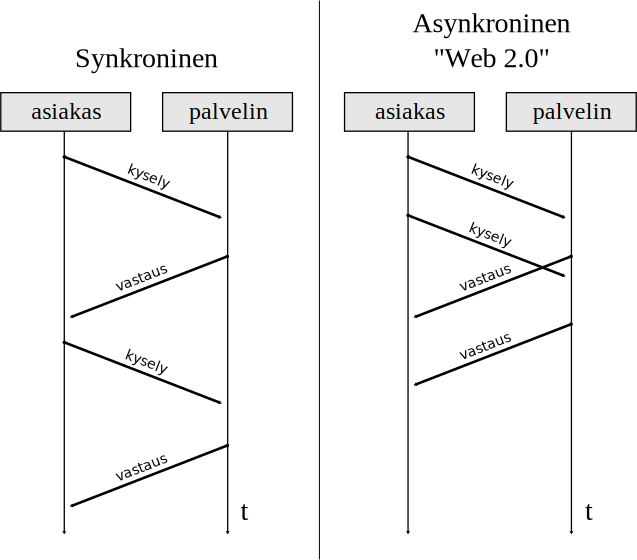
\includegraphics[width=11.5cm]{pics/synkroninen.pdf}
\caption{Synkroninen ja asynkroninen kommunikointi.}
\label{synkroninen}
\end{figure}

AJAXiin kohdistuvat hyökkäykset eivät eroa suuresti vanhoista murtautumismenetelmistä. Hyökkääjät pyrkivät edelleen hyödyntämään syötteen puutteellista suodattamista, muokkaamaan 
ulos tulevaa dataa, murtamaan salauksia ja hankkimaan istuntokohtaisia tietoja esimerkiksi evästeitä varastamalla. Hyökkääjien näkökulmasta AJAXin tekee erityisen kiinnostavaksi se,
että aiempaa suurempi osa Web-palvelun käyttämästä laskennasta suoritetaan käyttäjän selaimessa. Käyttäjän selaimeen, eli ns. asiakaspuoleen, ei voida kuitenkaan koskaan luottaa.
JavaScriptien huolimaton käyttö avaakin hyökkääjille lukuisia tapoja murtautua palveluihin. Kyseessä on sinänsä pitkään tunnettu ongelma, mutta kehittäjien kiinnostuksen siirtyessä 
AJAXiin ovat myös hyökkääjät alkaneet kiinnittämään asiaan enemmän huomiota \cite{AJAX}. Monet käytetyistä AJAX-ympäristöistä sisältävät myös eriasteisia tietoturvariskejä, joita 
hyökkääjät voivat hyödyntää \cite{JSH}.

\subsection{JavaScript}

JavaScript on Netscapen suunnittelema skriptikieli, joka tunnettiin aluksi nimellä LiveScript. Sun Microsystemsin kehittämän Java-ohjelmointikielen yleistyessä Netscape päätti muuttaa
sen nimen JavaScriptiksi toivoen sen käytön yleistyvän Javan menestyksen myötä. JavaScriptillä kirjoitetut skriptit sijoitetaan HTML:n \texttt{<script>}-elementin sisään, josta voi 
olla myös viite erilliseen lähdekooditiedostoon. JavaScript vaatii tuen selaimelta, jollainen löytyy miltei jokaisesta Web-\-selaimesta mukaan lukien yleisimmät mobiililaitteet.

JavaScript on tehokas työkalu, joka mahdollistaa monen muun toiminnon ohella muun muassa dynaamisten Web-sivujen tekemisen, viestien kirjoittamisen selaimen tilariville, uusien ikkunoiden
avaamisen ja interaktiivisten lomakkeiden luomisen. Skriptien toiminta rajoittuu kuitenkin Web-selaimen toimintoihin, eikä sitä käyttäen voida esimerkiksi kirjoittaa levylle ja levyn 
lukeminen rajoittuu pelkästään evästeisiin \cite{JavaScript}. Näistä rajoituksista huolimatta JavaScript mahdollistaa erittäin monipuolisten toimintojen toteuttamisen Web-ympäristössä.

Suurin osa Web-sivuilla olevista skripteistä toimii siten, että ne ladataan aluksi käyttäjän koneelle, jonka jälkeen ne suoritetaan selaimessa. Skriptit sijaitsevat ja ne suoritetaan 
käyttäjien koneilla, joten toimintaperiaatteen selvittäminen ei ole hyökkääjälle vaikeaa. Asiaa pystytään kuitenkin vaikeuttamaan muutamalla eri tavalla. Näistä yksinkertaisin on 
\emph{obfuskointi}, jonka yhteydessä koodista tehdään vaikeasti luettavaa. Aluksi poistetaan kommentointi ja tyhjät rivivälit, seuraava askel on koodin muuttujien ja objektien
uudelleen nimeäminen, jolloin hyökkääjän on vaikeampi päätellä näistä skriptin toimintaperiaate. Nimet voidaan myös muuttaa esimerkiksi binäärikoodiksi. Nämä keinot ovat kuitenkin 
vain hidasteita osaavalle hyökkääjälle \cite{AJAX}. Palvelu tulisikin suunnitella siten, että kaikki luottamuksellisen tiedon käsittely ja käyttäjän syötteen tarkistukset suoritettaisiin
Web-palvelimella. Tällöin käyttäjän selaimessa suoritettaisiin ainoastaan sellainen laskenta, joissa käsitellään käyttäjää itseään koskevaa dataa.

Koneelle ladatut skriptit ajetaan oletuksena hyvin rajatussa tilassa, jossa niillä on pääsy vain kyseistä sivun sisältämään dataan tai siihen hyvin läheisesti kuuluviin dokumentteihin. 
JavaScript noudattaa myös  edellisessä luvussa esitettyä \emph{saman alkuperän} periaatetta, joka estää skriptien suorittamisen muista Internet-domaineista kuin siitä, josta skripti on
ladattu. Näin vaikeutetaan hyökkäyksen tekemistä käyttäen toiselta sivulta ladattua haitallista skriptiä, jonka avulla voitaisiin esimerkiksi varastaa evästeitä ja urkkia näppäimistön
painallukset.  Aikaisemmin selaimet ovat sallineet joitain poikkeuksia tähän periaatteeseen, mutta tietoturvasyistä nämä on kuitenkin poistettu.

Liian tiukat tietoturvasäännöt eivät 
kuitenkaan toimi nykyaikaisten Web-\-palveluiden kanssa, ja tästä syystä \emph{saman alkuperän} periaatetta on mahdollista löysentää. Esimerkiksi ulkoiset linkit, jotka osoittavat toisella
sivustolla olevaan skriptiin, ohittavat \emph{saman alkuperän}, sillä vaikka itse skripti sijaitsee toisella palvelimella niin se lasketaan kuuluvan siihen sivuun, jossa viittaus
lähdekooditiedostoon on.  Näin kutsutulla skriptillä on pääsy sellaisiin evästeisiin ja tiedostoihin, joihin sillä ei välttämättä tarvitsisi olla oikeuksia. Sivustojen ja palveluiden 
käyttäessä resursseja entistä useammasta lähteestä eri palvelimilta, voi tämä aiheuttaa riskitilanteita, jos jonkin lähteen tietoturva on vaarantunut \cite{AJAX}.

\subsection{AJAXiin liittyvät tietoturvariskit}

Koska AJAXin toiminta perustuu hyvin pitkälti JavaScriptin varaan, on itsestään selvää, että hyökkääjät pyrkivät väärinkäyttämään ensisijaisesti JavaScriptin haavoittuvaisuuksia.  
Asiaa ei auta se, että suurin osa sivustoista on jollakin tavalla alttiina XSS-hyökkäyksille \cite{WEB2c} johtuen huonosti toteutetusta syötteen tarkistuksesta. Asetettuja suodatuksia 
pystytään myös kiertämään käyttäen esimerkiksi kuvalinkkejä ja monia HTML-elementtejä, joiden avulla ajettava skripti voidaan hukuttaa muun syötteen joukkoon. Tästä syystä pelkästään 
tiettyjen merkkijonojen suodattaminen ei takaa suojaa JavaScript-pohjaisilta hyökkäyksiltä. Tehokkain ja yksinkertaisin keino onkin poistaa kaikki HTML-elementteihin kuuluvat merkit, 
jolloin esimerkiksi \texttt{<}-merkistä tulee \texttt{\&lt;} ja \texttt{>}-merkistä \texttt{\&gt;}. Monet ympäristöt mahdollistavat myös suoraan HTML-elementtien poistamisen käyttäjien
jättämistä viesteistä \cite{AJAX}. Tällöin esimerkiksi foorumeilla toisten käyttäjien lähettämistä viesteistä saadaan estettyä niiden mahdollisesti sisältämän JavaScript-ohjelmakoodin
suorittaminen.

Kasvaneella JavaScriptin käytöllä on suora vaikutus myös XSS-hyökkäysten yleistymiseen. JavaScriptillä pääsee helposti evästeisiin käsiksi käyttäen \emph{document.cookie}-oliota. 
Vaikka sen käyttö on rajoitettu ainoastaan sen Internet-domainin evästeeseen, josta kutsu on tehty, voidaan tämä rajoitus ohittaa melko helposti. Hyökkääjälle riittää, että käyttäjä 
vierailee esimerkiksi sellaisessa foorumissa tai blogissa, joissa käyttäjien viesteissä sallitaan XHTML:n käyttö. Tämä mahdollistaa haitallisten skriptien lähettämisen sivustolle ja pahaa
aavistamaton käyttäjä, joka vierailee tällä sivulla, joutuu tietämättään hyökkäyksen kohteeksi.

Yksi tapa suojautua evästeiden varastamiselta on käyttää HTTP-only~-evästeitä, jolloin asiakaspuolen evästeitä ei pystytä lukemaan. Näiden evästeiden tukeminen on kuitenkin selainkohtaista,
joten tämä ratkaisu ei aina välttämättä ole mahdollista toteuttaa. XSS-hyökkäykset eivät myöskään rajoitu pelkästään evästeiden varastamiseen, ja yhtä helposti hyökkääjä voi esimerkiksi
luoda skriptin, joka lukee näppäimistön painallukset ja lähettää ne haluttuun osoitteeseen. HTTP-only -evästeiden käyttö ei myöskään täysin suojaa evästeitä, jos käytetään XHR-kutsuja. 
Tällöin hyökkääjän on mahdollista lukea suoraan otsaketiedoissa asetettuja arvoja. Jotkut XHR-objekteihin liittyvät haavoittuvuudet ovat myös niin syvällä XHMLHttpRequest-objekteissa, että 
kaikki nykyisin käytössä olevat toteutukset ovat niille jossakin määrin alttiina. Kaapattujen XHR-objektien tunnistaminen ei myöskään vielä ole mahdollista \cite{AJAX}. Näistä syistä johtuen 
AJAX tarjoaa nyt ja tulevaisuudessa hyökkääjille monia mahdollisuuksia murtaa asetettuja suojauksia.

Yksi yleisimmistä AJAXissa käytetyistä dataformaateista on JavaScript Object Notationt (lyh. JSON). Se on ohjelmointikielestä riippumaton ja laajasti tuettu Web-palvelimella käytetty 
työkalu. Se on rakenteeltaan hyvin kevyt ja se koostuu kahdesta eri tietotyypistä: olioista ja taulukoista \cite{JSON}. Formaatin heikkous piilee siinä, että JSON-olio itsessään on kelvollinen 
JavaScript-ohjelma, jonka sisältö on mahdollista kaapata \cite{AJAX}. Termi \emph{JavaScript Hijacking} kuvaa tällaista tilannetta, jossa hyökkääjä ohittaa \emph{saman alkuperän} periaatteen 
silloin, kun JavaScriptiä käytetään arkaluontoisen tiedon lähettämiseen. Aiheesta tehdyn tutkimuksen \cite{JSH} mukaan lähes jokainen käytetty AJAX-ympäristö on alttiina tällaisilla hyökkäyksille.
Käyttäen CSRF-hyökkäystä hyökkääjä pystyy väärinkäyttämään JSON-formaattia, ja varastamaan sekä muokkaamaan toiselle sivustolle lähetettäviä paketteja.  Tällainen hyökkäys voidaan toteuttaa 
useilla eri tavoilla mukaan lukien käyttäen \texttt{<script>}-elementtiä, ja koska pyyntö tulee selaimen luottamasta lähteestä, voidaan tällä tavoin ohittaa esimerkiksi SSL-suojaus\cite{AJAX}.

Suojautuminen tämän tyyppisiltä hyökkäyksiltä voidaan toteuttaa monella eri tapaa, ja paras tulos saadaan yhdistelemällä näitä. Koska CSRF-hyökkäyksessä hyökkääjä joutuu toimimaan osittain 
sokeasti, voidaan jokaiseen pyyntöön lisätä parametri, jota hyökkääjän on vaikea arvata. Palvelin voidaan myös asettaa tarkistamaan HTTP Referer -kenttä, jolla voidaan varmistaa, että pyyntö 
tulee sallitulta taholta, vaikkakin Referer-kentän sisältö voidaan helposti muuttaa. Toinen tapa on muokata vastaanottopäässä paketteja siten, että hyökkääjä ei pysty ajamaan lähettämissään 
pyynnöissä skriptejä 
\cite{JSH}.

\section{Flash}

AJAXin ohella Macromedian suunnittelema, ja nykyisin Adoben kehittämä Flash, on ollut yksi niistä merkittävistä tekniikoista, joita käyttämällä YouTuben ja MySpacen kaltaiset 
menestyspalvelut ovat olleet mahdollisia toteuttaa. Flashia käyttämällä kehittäjät ovat jo pitkään pystyneet luomaan interaktiivista ja rikasta Web-sisältöä
yksinkertaisista animaatioista aina monimutkaisiin peleihin ja valikoihin asti. Suurin osa Web-sivustoilla olevista mainoksista on myös toteutettu käyttäen Flashia. Näistä syistä johtuen 
Flash Player on yksi ohjelmistoalan de facto~-tekniikoista, jonka käyttöaste yritys- ja kuluttajapuolella on lähes 100 prosenttia \cite{Flash}.

Flashin käyttämä ActionScript-skriptikieli muistuttaa läheisesti JavaScriptiä ja sitä käyttäen on mahdollista luoda uusia TCP-yhteyksiä, ajaa JavaScriptiä selaimessa ja luoda 
sallittuihin domaineihin HTTP-pyyntöjä. Flashin käyttämä tietoturvamalli noudattaa paljolti \emph{saman alkuperän} periaatetta, jolla rajoitetaan eri domaineissa sijaitsevien sovellusten 
kommunikointia. Domainien välinen kommunikointi on kuitenkin sallittua, ja käytetty tietoturvapolitiikka luetaan tähän tarkoitetusta XML-tiedostosta. Tämä XML-tiedosto sijaitsee usein 
domainin juuressa ja se sisältää ne domainit, jotka saavat olla siihen yhteydessä. Osa Flashiin kohdistuvista hyökkäyksistä pyrkiikin muokkaamaan tietoturvapolitiikkatiedoston sisältöä
siten, että kohde sallisi yhteydet myös hyökkääjän käyttämästä osoitteesta. Tämä voidaan toteuttaa esimerkiksi käyttämällä vihamielistä RSS-syötettä tai luomalla tiedosto, joka sisältää
uuden XML-tiedoston. Yksi tällaisista hyökkäyksistä on Stefan Esserin luoma GIF-tiedosto, jonka kommenttiin on piilotettu uusi tietoturvapolitiikka. Hyökkääjälle riittää, että kohdekone 
vain mahdollistaa tiedoston lataamisen palvelimelle, jonka jälkeen vanha sisältö voidaan korvata GIF-tiedostoon piilotetulla \cite{WEB2}.

Perimmäinen syy sille, miksi XSS-hyökkäykset ovat yleistyneet viime vuosina on se, että käyttäjien antamaa syötettä ei usein tarkisteta riittävällä tarkkuudella. Sama pätee myös suureen 
osaan Flash-pohjaisista toteutuksista, joihin käyttäjien on mahdollista antaa syötteitä. Tämä avaa useita erilaisia Flashia hyödyntäviä XSS-hyökkäyksiä, jotka pyrkivät väärinkäyttämään 
käyttäjän selaimen ja sivuston välistä luottamussuhdetta. Aina vika ei ole Flash-toteutuksen tekijässä, sillä Flash-tiedostoja luodaan usein automaattisesti käyttämällä valmiita 
sovelluksia. Aiheesta tehdyn kattavan tutkimuksen mukaan \cite{FlashXSS} suurimmasta osasta näin luoduista tiedostoista löytyy XSS-haavoittuvaisuuksia, jotka mahdollistavat JavaScriptin
ajamisen siinä domainissa, jossa haavoittuvainen SWF-tiedosto sijaitsee. Osa näistä tietoturvaongelmista on myöhemmin korjattu tutkimuksen julkaisun jälkeen, mutta tehty tutkimus osoittaa 
sen, että edes luotettavina pidettävien tahojen toteutuksiin ei pidä luottaa liikaa.

Yksi käytetyimmistä Flash-pohjaisista toteutuksista ovat erilaiset interaktiiviset mainokset, joita löytyy lähes jokaiselta sivustolta. Flashin levinneisyyden ansiosta ne toimivat miltei
jokaisella käyttäjällä ja siksi ne ovat houkutteleva keino toteuttaa hyökkäyksiä. Adobe Flash Playerista on löydetty useita eri haavoittuvaisuuksia, jotka ovat mahdollistaneet haitallisten
koodien ajamisen kohdekoneessa. Flash-mainoksia käytetään myös laajalti haittaohjelmien levittämiseen, ja usein tällä tavalla altistuneet koneet kuuluvat käyttäjän tietämättä 
bottiverkkoihin, joita käytetään roskapostin lähettämiseen ja palvelunestohyökkäyksiin. Haitallista koodia sisältävä mainos voi myös esimerkiksi pyrkiä ohjaamaan selaimen toiselle 
sivustolle käyttäen ActionScriptia.  Tällaiset haitalliset mainokset eivät ole pelkästään vain pienten sivustojen ongelma, sillä vuonna 2009 suuret sivustot kuten \emph{guardian.co.uk} 
sisälsivät mainoksia, jotka olivat luonteeltaan haitallisia \cite{FlashAdd}.

\section{Google Web Toolkit}

Nykyisin yhä useampi taho pyrkii hyödyntämään tekniikoita kuten AJAXia ja JavaScriptiä omissa web-palveluissaan, ja tulevaisuudessa tämä kasvu tulee vain jatkumaan. Toimivien ja 
turvallisten  Web-palveluiden suunnitteleminen ja toteuttaminen vaatii kuitenkin sellaista syvällistä tietämystä käytetyistä tekniikoista, jota harvemmin suunnittelijoilta löytyy. 
Tämä on yksi  niistä pääsyistä, jonka takia Web-pohjaiset hyökkäykset ovat kasvaneet määrällisesti suurimmaksi hyökkäystavaksi. Asian helpottamiseksi on kehitetty erilaisia 
kehitysympäristöjä, jotka pyrkivät helpottamaan suunnittelijoiden taakkaa, ja samalla tarjoamaan jonkinlaista tietoturvaa. Yksi tällaisista on Googlen kehittämä Google Web Toolkit, 
joka on kasvamassa yhdeksi käytetyimmistä uusista kehitysympäristöistä.

\subsection{Google Web Toolkit lyhyesti}

Google Web Toolkit (lyh. GWT) on avoimeen lähdekoodiin perustuva kehitysympäristö rikkaiden ja dynaamisten Web-sovellusten kehittämiseen. Suunnittelun lähtökohtana on ollut mahdollistaa
korkealaatuisten Web-sovellusten tehokas suunnittelu ilman, että kehittäjän tulee olla asiantuntija niin selainten pienissä kummallisuuksissa kuin myös XMLHttpRequest- pyyntöjen
tekemisessä ja JavaScriptien kirjoittamisessa. Tämä on mahdollista, koska GWT:llä AJAX-sovellukset kirjoitetaan Javalla, joka mahdollistaa keskittymisen korkeamman tason suunnitteluun 
ilman, että aikaa tuhlaantuisi DOM- ja XHR-kutsujen säätämiseen. Valmis Java-sovellus käännetään automaattisesti JavaScriptiksi, ja samalla skriptien sisältö optimoidaan muun muassa
poistamalla käyttämättömät muuttuja ja parametrit. Tämän ratkaisun etuna on myös se, että kehittäjät voivat käyttää haluamaansa Java-ympäristöä sovellusten kirjoittamiseen ja koodin 
tarkistamiseen. Käännetyt JavaScriptit myös toimivat suoraan suurimmassa osassa selaimista sekä Androidissa ja iPhonessa \cite{GWT}.

\subsection{Google Web Toolkitin ominaisuuksia}

GWT 2.0 on uusin versio ympäristöstä ja se on tuonut mukanaan suuren joukon uusia ominaisuuksia vanhoihin versioihin verrattuna. Yksi tärkeimmistä on niin kutsutun ``hosted moden'' 
korvaaminen \emph{GWT Developer} liitännäisellä. Hosted mode oli yksi GWT:een kantavista ideoista, joka mahdollisti tietyn selainympäristön emuloimisen. Hosted modea käyttäen 
kehittäjällä oli mahdollisuus kirjoittaa Java-koodia ja tutkia sen toimivuutta Web-selaimessa ilman, että koodia piti kääntää JavaScriptiksi. Tämä säästi reilusti kehittäjän aikaa, sillä 
ison koodin kääntäminen on aina hidasta. Tämän ratkaisun ongelmana oli se, että emuloidut ympäristöt edustivat vanhoja selainversioita, eikä selaimille jo valmiiksi kirjoitettuja 
testausohjelmia kuten Firebugia pystynyt käyttämään. Käyttäen Developer pluginia kehittäjien on nyt mahdollista ajaa ja testata koodia suoraan suosituimmilla selaimilla, jolloin esimerkiksi
tyylitiedostojen säätäminen on helpompaa. Koodin testaaminen yhtäaikaisesti useammalla eri selaimella on myös mahdollista \cite{GWTnew}. 

Toinen suuri uudistus GWT 2.0:ssa on mahdollisuus pilkkoa ajettava koodi pienempiin osiin (Code Splitting). Nykyisten AJAX-sovellusten ongelmana on se, että sivun sisältö pitää lähes aina 
ladata kokonaan selaimeen, ennen kuin palvelua voidaan käyttää. Sivustojen kasvaessa entistä suuremmiksi tämä kasvattaa käyttäjien kokemaa viivettä, ja yksi AJAXin eduista on juuri
viipeen vähentäminen. Pilkkomalla ajettava komentosarja pienempiin osiin käyttäen valmista funktiota, voidaan tämä ongelma välttää kokonaan. Riittää, että kehittäjä määrittää ne kohdat, 
jotka hän haluaa ladattavan pienemmissä osissa. Tällä tavoin voidaan esimerkiksi ladata ensiksi käyttöliittymä ja yleisimmin käytetyt valikot, ja vasta käytön aikana ladata vähemmän 
käytetyt toiminnot. GWT pitää myös itse huolen siitä, että kaikki tarvittavat riippuvuudet ladataan oikessa järjestyksessä \cite{GWTnew}

\subsection{Google Web Toolkitin tietoturva}

Koska GWT:n lopputuotos on JavaScriptiä, on se periaatteessa samalla tavalla haavoittuvainen hyökkäyksille kuten Cross-Site Scriptingille ja Cross-Site Request Forgerylle. Yleisellä tasolla 
GWT:een tuottama JavaScript-komentosarja noudattaa hyväksi todettuja käytäntöjä, jotka vähentävät riskiä joutua tällaisten hyökkäysten kohteeksi. On kuitenkin asioita, joihin kehittäjien tulee edelleen
kiinnittää tarkkaa huomiota. 

Ensimmäinen näistä on olla käyttämättä omia ja kolmannen osapuolen skriptejä sekaisin. Tiettyjen toimintojen kuten innerHTML:n ja eval-funktion kanssa tulee myös olla erittäin tarkkana.
Esimerkiksi innerHTML-atribuuttia käytetään usein staattisen HTML-sisällön tuomiseen JavaScript-objektin määrittämiin valmiisiin taulukoihin ja ikkunoihin. Tämän tekniikan käyttäminen on 
kuitenkin riskialtista, sillä se mahdollistaa haitallisen koodin sisällyttämisen suoraan sivustolle. Mihinkään syötteeseen ei pidä myöskään koskaan luottaa suoraan, vaikka se tulisi omalta 
palvelimelta erityisesti jos se on menossa innerHTML- tai eval-funktioiden käyttöön. Sama pätee myös JSON-syötteisiin, joiden avulla on mahdollista suoraan ajaa haitallista JavaScriptiä, jos 
syötettä ei tarkisteta riittävällä tarkkuudella. Tärkeintä onkin aina tarkistaa erittäin tarkasti eri syötteet riippumatta siitä, mikä osapuoli sen on lähettänyt ja mihinkä käyttöön se on
menossa \cite{GWTsecurity}.

CSRF-hyökkäykset kohdistuvat aina palvelinpuolen huonosti toteutettuun sessionhallintaan, jossa pyynnön tehneen tahon oikeellisuutta ei varmisteta. Määrittämällä JavaScript kopioimaan aina 
sessiossa käytetyn evästeen arvo jokaiseen kyselyyn mukaan, voi palvelin verrata tätä arvoa luomaansa evästeeseen. Koska \emph{saman alkuperän} periaate estää kolmannen osapuolen sivustoa 
pääsemästä käsiksi tähän evästeeseen, voi palvelin olla varma, että pyynnön on todellakin tehnyt käyttäjä itse. GWT:stä löytyy valmiiksi tähän tarkoitukseen kirjoitettuja funktioita, joita
käyttäen jokaiseen pyyntöön voidaan lisätä oikean evästeen arvo. Näitä käyttäen CSRF-hyökkäykset voidaan lähes kokonaan poistaa, kunhan vain palvelinpuoli osaa verrata evästeiden arvoja 
ja tehdä näiden pohjalta oikeat johtopäätökset. JSONin tapauksessa voidaan tämän lisäksi käyttää jo aikaisemmin esitettyä tapaa, jossa pakettien sisältöä muokataan siten, ettei niiden
sisältöä voida kaapata käyttäen <script>-elementtiä \cite{GWTsecurity}.

% FIXME onko hyvä tuo <script> ?

% -*- mode: LaTeX; coding: utf-8; -*-

\chapter{Aiheeseen liittyvä tutkimus}

\section{Yleistä}

Viime vuosina web-sovellukset ovat kasvattaneet suuresti suosiota, ja nykyisin yhä useampi palvelu, jossa tietoturvan ja saatavuuden takaaminen on elintärkeää, on siirtynyt osittain tai kokonaan 
verkon puolelle. Tämä on vaikuttanut suuresti siihen, mihin tietoturvahyökkäykset nykyisin kohdistuvat ja kuinka niitä pyritään toteuttamaan. Hyökkäysten muuttuessa yhä hienostuneimmiksi, 
eivät perinteiset tietoturvamenetelmät enää riitä suojaamaan loppukäyttäjiä tai palvelun ylläpitäjiä. Tästä syystä erilaisten tietoturvaratkaisuiden ympärillä käy kova kuhina, ja aihepiiri 
onkin herättänyt suurta kiinnostusta tutkijoiden keskuudessa. Erilaisia ratkaisuja, joissa on pyritty selvittämään aikaisemmissa luvuissa esitettyjä tietoturvahyökkäyksiä ja näiden 
mukana tulleita haasteita, on lukematon määrä. Seuraavaksi esitellyt tutkimukset edustavat vain pientä osaa koko tutkimuskentästä, mutta näistä käy kuitenkin jo ilmi se, millaisiin ratkaisumalleihin
nykyisin pyritään.

Hyökkäysten tunnistaminen toimii siten, että analysoimalla yhtä tai useampaa tapahtumaa pyritään löytämään viitteitä tapahtuvista hyökkäyksistä. Tunnistamiseen pohjautuvat menetelmät jaetaan usein
kahteen eri tyyppiin: anomalioiden eli poikkeavuuksien tunnistamiseen (eng. anomaly detection) ja väärinkäytösten tunnistamiseen (eng. misuse detection). Näistä anomalioiden tunnistamiseen perustuvat
järjestelmät luovat malleja järjestelmän, käyttäjän tai verkon normaalista käyttäytymisestä, ja vertaamalla tapahtumia näin muodostettuihin kuvauksiin voidaan poikkeavuudet tunnistaa. Väärinkäytösten 
tunnistamiseen tarkoitetut järjestelmät taas sisältävät joukon kuvauksia eli signatuureja tunnetuista hyökkäyksistä. Tuleva liikenne tarkistetaan näitä kuvauksia vastaan, jolloin kuvauksia vastaavat
hyökkäykset voidaan tunnistaa. Joissakin tapauksissa jaottelu on myös tehty sen mukaan, mistä tutkittava liikenne on kerätty. Tällöin järjestelmät on jaettu verkkoon pohjautuviksi (eng. network based)
ja asiakaspohjaisiksi (eng. host based). 

\section{Väärinkäytösten tunnistaminen}

Väärinkäytökseen perustuvat järjestelmät ovat pitkään olleet suosituin lähestymistapa hyökkäysten torjumisessa. Nämä järjestelmät on voitu jakaa kahteen erilliseen osaan, jossa tilattomassa 
järjestelmässä jokaista tulevaa tapahtumaa käsitellään itsenäisesti, kun taas tilallisessa järjestelmässä tutkitaan tapahtumien välisiä suhteita. Web-pohjaisten hyökkäysten tutkimisessa tietolähteinä 
on käytetty mm. palvelimien tuottamaa lokia \cite{LightTool} ja IDS-järjestelmien \cite{Snort}\cite{Bro} tapauksessa analysoimalla verkkokerroksen liikennettä. Ensimmäisessä ratkaisussa ongelmana
on, että itse palvelimiin kohdistuvia hyökkäyksiä ei pystytä havaitsemaan ainoastaan lokitietoa tarkkailemalla. Samoin hyökkäyksiä, jotka koostuvat monista eri vaiheesta, on mahdotonta mallintaa. 
Verkkokerroksella toimivia järjestelmiä taas pystytään harhauttamaan muokkaamalla hyökkäyksiä, ja näistä harvat mahdollistavat tilallisen analyysin. 

Esitettyjä ongelmia on pyritty ratkaisemaan lisäämällä havaittavien tapahtumien määrää ja keräämällä informaatiota eri lähteistä. Esimerkiksi asentamalla sovellustasolle erillinen tiedonkeruuseen 
tarkoitettu komponentti \cite{Application} on saatu hyviä tuloksia. Tässä tapauksessa tiedonkeruu tapahtui Apache-palvelimelle asennetun komponentin välityksellä, joka tarkkaile lokitiedon lisäksi
mm. pyyntöjen tulkitsemiseen ja toteuttamiseen menevää aikaa. Tämän ratkaisun etuna on myös se, että tutkittava data on salaamattomassa muodossa ja sessioiden uudelleenrakentaminen on mahdollista. 
Tällä tasolla toimiva IDS-järjestelmä voi myös toimia ennaltaehkäisevästi eli haitalliseksi havaittu liikenne voidaan tiputtaa pois ennen kuin se käsitellään palvelimella. Suurimpana haittapuolena on, 
että tietylle sovellukselle suunniteltua komponenttia ei voida sellaisenaan käyttää muilla alustoilla. 

WebSTAT \cite{Webstat} on tilalliseen analyysiin perustuva IDS-järjestelmä, joka pohjautuu STAT-kehitysympäristöön \cite{STAT}. WebSTAT hyödyntää STATL-ohjelmointikieltä, joka mahdollistaa hyökkäysten
mallintamisen ottamalla huomioon mm. eri tapahtumien välisiä yhteyksiä ja verkkohistoriaa sekä palvelimien kuten Apachen ja Microsoftin IIS:n lokia. Koska tietoa kerätään yhtäaikaisesti monesta eri 
lähteestä, voidaan palvelimien lokitiedon analysointiin yhdistää alempien toimintojen kuten jär\-jes\-tel\-mä- ja verkkotason tuottamaa tietoa. Näin tehty analyysi kuvaa koko järjestelmä tilaa, jolloin 
yllättävät muutokset pystytään havaitsemaan nopeasti. Testien mukaan tällainen analyysi voidaan toteuttaa suurissa järjestelmissä reaaliajassa aiheuttamatta suurempaa viivettä palvelimien toiminnassa. 
Menetelmän sovittaminen tiettyyn järjestelmään vaatii jonkin verran manuaalista työtä, ja tätä voidaankin pitää sen suurimpana heikkoutena. Monimutkaisten hyökkäysten kuvaaminen on usein myös hankala
toteuttaa, ja niiden tulkitsemiseen saattaa tuhlaantua turhaa aikaa.

Väärinkäytösten tunnistamiseen tarkoitettuja järjestelmiä on hyödynnetty myös uudempien tietoturvahyökkäysten tunnistamisessa. Esimerkiksi vihamielisten Flash-mainosten tunnistamiseen tarkoitettu 
OdoSwiff \cite{FlashAdd} pyrkii etsimään sivuilla olevista mainoksista hyökkäykseen tarkoitettua koodia käyttäen staattista ja dynaamista analyysia. Palvelinpuolella XSS-hyökkäyksiä vastaan on luotu 
järjestelmä, josta löytyy yleisimpien hyökkäysten kuvaukset \cite{SignatureXSS}. Kumpikin järjestelmistä toimii erittäin hyvin, kunhan hyökkäys on entuudestaan tuttu.

\section{Poikkeavuuksien tunnistaminen}

Väärinkäytösten tunnistamiseen käytettyjen järjestelmien suurin heikkous piilee siinä, että mallintamattomat hyökkäykset jäävät näiltä huomaamatta. Tämä on erityisesti web-palveluihin kohdistuvien
hyökkäysten tapauksessa iso ongelma, sillä toimintaympäristö muuttuu jatkuvasti, ja uusia hyökkäyksiä ja vanhojena variaatioita ilmestyy tiuhaan tahtiin. Tällöin signatuurien pitäminen ajantasalla
muodostuu mahdottomaksi tehtäväksi. Hyökkäysten monimuotoisuus onkin johtanut siihen, että nykyisin yhä useammassa järjestelmässä pyritään tunnistamaan poikkeavat tapahtumat normaaliin liikenteen seasta
ilman tarkkoja signatuureja. 

Anomalioiden tunnistamiseen on käytössä useita eri menetelmiä, ja ne voidaan jakaa kahteen eri ryhmään \cite{State}. Näistä ensimmäinen sisältää oppimiseen pohjautuvat mallit, jossa normaali 
käyttäytyminen opetetaan opetusmateriaalin avulla. Normaalia käyttäytymistä esittävät profiilit voidaan mallintaa käyttäen joko sään\-tö\-poh\-jais\-ta-, mallipohjaista- tai tilastopohjaista menetelmää. Näistä
sääntöpohjaiset menetelmät muistuttavat eniten perinteisiä IDS-järjestelmiä sillä erolla, että luodut säännöt pohjautuvat kerättävään dataan, ja säännöt voivat olla rakenteiltaan hyvin monimutkaisia. 
Mallipohjaisissa menetelmissä taas luodaan normaalia käyttäytymistä kuvaavat profiilit, jota vastaan tuleva liikenne arvioidaan. Tiedonlouhinta, neuroverkot ja liikenteestä luotujen kuvioiden vertaaminen
tulevaan liikenteeseen (eng. pattern matching) ovat tekniikoita, joita on käytetty tällaisten mallien luomiseen. Analyysissa voidaan esimerkiksi tutkia verkkopakettien kuormia \cite{Payload}\cite{ULISSE} 
ja klusteroimalla ja luokittelemalla liikenne protokollien ja palveluiden mukaan \cite{Cluster}. Viimeisen ryhmän muodostavat tilastollisiin menetelmiin pohjautuvat menetelmät \cite{PacketHeader}, jotka
ovat jääneet vähemmälle huomiolle johtuen alati muuttuvasta toimintaympäristöstä.

Toisen ryhmä anomalioiden tutkimisessa muodostavat spesifistiset mallit (eng. spesification model). Nämä menetelmät pohjautuvat enemmän ihmisten huomioihin ja asiantuntijuuteen kuin matemaattisiin
kuvauksiin. Menetelmissä käytetään useita eri elementtejä aina sovellustasolta verkkotasolle, ja näitä käyttäen luodaan normaalia käyttäytymistä kuvaavat mallit. Järjestelmät voivat hyödyntää esimerkiksi
protokollista kerättävää tietoa anomalioiden tunnistamisessa. Järjestelmien eri tiloja ja tapahtumien välisiä suhteita voidaan myös mallintaa, jolloin poikkeavat tilat ja tapahtumaketjut voidaan
tunnistaa. 

Anomalioiden tunnistamiseen perustuville järjestelmille löytyy useita eri käyttökohteita. Niillä voidaan esimerkiksi pyrkiä tunnistamaan tietokantoihin kohdistuvia tunnettuja ja tuntemattomia SQL-hyökkäyksiä.
Järjestelmälle voidaan opettaa normaali käyttäytyminen esimerkiksi tiedonlouhintamenetelmin \cite{Data} tai luomalla profiileja normaalista käyttäytymisestä \cite{SQLanomaly}\cite{SQLlearning}. Erilaisia
menetelmiä voidaan myös yhdistellä, jolloin todennäköisyys poikkeavan liikenteen tunnistamiseen kasvaa. Tutkimalla esimerkiksi yhtä aikaisesti sekä web-pyynnöissä että SQL-kyselyissä ilmeneviä poikkeavuuksia, 
voidaan tulevat kyselyt pisteyttää tarkasti \cite{WebSQL}. Kyselyiden kategoriointi mahdollistaa sen, että haitalliseksikin merkityt kyselyt voidaan ohjata sellaisille palvelimille, joilla ei ole 
pääsyä arkaluontoiseen tietoon. 

Web-palveluihin kohdistuvien hyökkäysten tunnistaminen on hankala ja aikaa vievä prosessi. Aikaisemmin tässä työssä esitetyt hyökkäykset kattavat vain osan hyökkäyksistä, joita vastaan sovellussuunnittelijat ja
ylläpitäjät joutuvat suojautumaan. Juuri tämä hyökkäysten monimuotoisuus on se seikka, joka on nostanut anomaliatutkimuksen muiden menetelmien yläpuolelle, ja aihepiiri on viime vuosina noussut yhdeksi 
puhutuimmista tietoturvan saralla. 

Poikkeavan tilan tunnistamiseen on käytetty monia eri menetelmiä, ja päätöksen tekemiseen on käytetty useita eri tietolähteitä. Esimerkiksi Swaddler \cite{Swaddler} on 
web-sovelluksille suunniteltu menetelmä, joka oppii kriittisten järjestelmäkutsujen ja sovelluksen tilojen väliset suhteen analysoimalla web-sovelluksen sisäisiä tiloja. Tällä tavoin voidaan tunnistaa hyökkäykset,
jotka aiheuttavat poikkeavia tiloja esimerkiksi sovelluksen normaaliin työkulkuun. Järjestelmä koostuu eri malleista ja osista, joille opetetaan harjoittelujakson aikana sitä vastaava normaali käytös. Jokaiselle
osalle, jotka käytännössä vastaavat tiettyjä sovelluksen toimintoja, lasketaan myös kynnysarvo, jonka ylittyessä sen aiheuttanut toiminto lasketaan anomaliaksi. Tehdyissä testeissä järjestelmä tunnisti 
kaikki toteutetut hyökkäykset, ja virheellisten positiivisten hälystysten määrä oli kohtuullisen pieni. Analysointi aiheutti jonkin verran kuormaa palvelimelle, mutta optimoimalla toteutusta tämä voidaan poistaa
lähes kokonaan. 

Aikaisemmin esitettyä tapaa, jossa hyödynnetään palvelimen tuottamaa logia, voidaan käyttää myös poikkeavuuksien tunnistamisessa \cite{Multi}. Tässä tapauksessa analysoitiin Apachen tuottamaa HTTP-logia, ja huomio kiinnitettiin kyselyihin, joissa parametreja käyttäen välitettiin arvoja palvelinpuolen ohjelmille tai aktivoitiin dokumentteja. Kyselyt purettiin osiin, ja niitä analysoitiin käyttäen useita eri malleja 
mm. kyselyjen pituutta ja normaalia järjestystä, merkkien jakaumia ja pyyntöjen tiheyttä. Vastaavaa mallia on sovellettu myös poikkeavien järjestelmäkutsujen tunnistamisessa \cite{SystemCall}, joten sen käyttö ei rajoitu pelkästään web-palveluihin. Väärinkäytös- ja anomaliamenetelmien yhdistämistä on myös ehdotettu \cite{Combination}. Tällainen järjestelmä voi toimia siten, että tuleva liikenne syötetään ensiksi anomalioita tutkivalle järjestelmälle, ja vain tunnistetut positiiviset tapaukset ohjataan väärinkäytösjärjestelmälle. Menetelmän etuna on, että virheellisten positiivisten määrä tippuu suuresti, ja tarkan analyysin vaativat tapahtumat pienenevät.



% -*- mode: LaTeX; coding: utf-8; -*-

\chapter{Tutkimusasetelma}

Edellisissä luvuissa on esitetty pieni osa niistä hyökkäyksistä, joita vastaan verkot ja web-palvelut joutuvat nykyisin suojautumaan. Niiden suuresta määrästä johtuen on ilmiselvää, että täysin 
turvallista ympäristöä on mahdoton rakentaa. Yleensä tämä ei ole edes tietoturvasuunnittelun lähtökohtana, vaan tärkeämpää on löytää tasapaino palvelun saatavuuden, ja käytettyjen tietoturvaratkaisuiden 
välillä. Liian raskaat menetelmät aiheuttavat ylimääräistä viivettä palvelun tai verkon saatavuuteen, ja liian kevyet ratkaisut jättävät ne avoimiksi yleisimmille hyökkäyksille. 

\section{Lähtökohta}
\label{sec:lahtokohta}

Tämän Pro gradu -tutkielman tavoitteena on pyrkiä tunnistamaan Web-palveluihin kohdistuvia poikkeavuuksia analysoimalla palvelimien tallentamaa tapahtumalokia.

Tässä tutkielmassa käytettävä data on peräisin Ixonos Oyj:ltä, joka tarjoaa muiden palveluidensa ohella hosting-palveluita suuryrityksille. Lokitiedostot ovat peräisin kolmelta tuotannosta jo poistetuilta palvelimilta, jotka ovat olleet vastuussa muutaman suuren palvelukokonaisuuden pyörittämisestä.

Analysoitava data on Apache-palvelimien tuottamaa lokia, joka sisältää
web-palveluille kohdistuvia HTTP-pyyntöjä. Lokia on yhteensä 24
gigatavua, ja se sisältää yli 1,7 miljardia sivupyyntöä, joista ??? on
tullut uniikista IP-osoitteesta. Lokia on kerätty noin 10 kuukauden
ajanjaksolta. 

% Tarkat luvut:
% - Dataa 24133108 kiB
% - Sivupyyntöjä (ml. error-logit) on 1666171347 kpl.

Loki on tallennettu \textit{Combined Log Format} -muodossa,
joka on yleinen Apache-palvelimen käyttämä lokitiedoston
muoto~\cite{combined}. Alla on esimerkki onnistuneen HTTP-kyselyn seurauksena muodostuneesta lokirivistä.

\begin{framed}
\begin{verbatim*}
130.234.49.2 - - [10/May/2009:15:53:01 +0300]
"GET /scripts/access.pl?user=matti&passwd=admin HTTP/1.1"
200 2680 "http://www.jyu.fi/a.html"
"Mozilla/5.0 (SymbianOS/9.2;...)"
\end{verbatim*}
\end{framed}

Web-palvelimien tuottama loki sisältää paljon tietoa muun muassa palveluiden käyttöasteista, ja niihin kohdistuvista kuormista. Niitä analysoimalla voidaan myös tunnistaa mahdollisia hyökkäysyrityksiä, sekä
hyökkäyksen jo tapahduttua tutkia siihen johtaneita vaiheita. Pienillä sivustoilla lokin läpikäyminen jälkikäteen käsin on vielä mahdollista, mutta puhuttaessa palveluista, joilla on miljoonia käyttäjiä 
kuukaudessa, ei tämä ole enää mahdollista. Tästä syystä lokien analysoiminen tulee automatisoida. Tämä taas johtaa siihen, että järjestelmän tulisi pystyä tunnistamaan miljoonien kyselyiden joukosta
ne, jotka ovat syntyneet hyökkäyksen johdosta. Yksi mahdollisuus on käyttää sääntöpohjaista ratkaisua, mutta aikaisemmin esitetyistä syistä johtuen, ei tämä tarjoa aina riittävää tunnistuskykyä. Tästä 
syystä olemme päätyneet käyttämään anomalioiden tunnistamismenetelmää, jossa järjestelmälle opetetaan normaali käyttäytyminen. Tämän jälkeen haluttu data verrataan opetettuun malliin, jolloin poikkeava
liikenne voidaan tunnistaa.

Tietoturvan kannalta kiinnostavin osa logista on GET-parametrin jälkeinen osa, jossa kuljetetaan varsinainen HTTP-pyyntö. Tämä sisältää niin staattiset sivunlatauspyynnöt, kuin myös palvelimelle 
välitettävät parametriarvot. Tällaisia voivat olla esimerkiksi kirjautumisessa käytetyt tiedot, ja tietokannalle välitetyt kyselyt. Staattiset sivunlatauspyynnöt ja parametreja sisältävät pyynnöt erottaa
resurssipolun jälkeisestä kysymysmerkistä. Kysymysmerkin jälkeinen kyselyosuus koostuu avain-arvo-pareista, joista ensimmäinen on kutsuttu parametri, ja jälkimmäinen tämän arvo (kuva \ref{CLF2}). Riippuen
palvelun toteutuksesta näitä voi olla useampia peräkkäin \&-merkillä erotettuna.

\begin{figure}[ht]
\centering
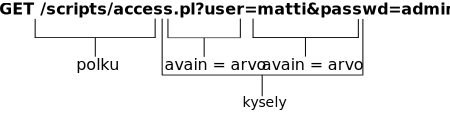
\includegraphics[width=13cm]{pics/logi2.pdf}
\caption{HTTP-kyselyn GET-osa}
\label{CLF2}
\end{figure}

\section{Käytettyjen menetelmien yleinen kuvaus}

Ongelmia lokin analysoimisessa aiheuttaa datan suuri määrä, ja lokissa esiintyvien parametrien tyypit. Näistä osa on luokka-asteikollisia ja osa puolestaan numeroasteikollisia, joten tietynlaisten toimintamallien 
etsiminen näistä on haastavaa. Parametrien suuri määrä aiheuttaa myös laskennallisia ongelmia, joten niiden määrää tulee pystyä jotenkin vähentämään säilyttäen kuitenkin mahdollisimman tarkkaan alkuperäisten muuttujien 
piirteet. Seuraavaksi esitetään yleisellä tasolla käytetyt tekniikat, ja sitä seuraa näiden tarkempi matemaattinen kuvaus.

Anomalioiden tunnistamiseen käyttämämme järjestelmä pohjautuu diffuusiokuvausten ja diffuusioetäisyyksien käyttöön, jotka tarjoavat tehokkaan tavan löytää merkittäviä geometrisia rakenteita datasta. Näiden
käyttämistä moniulotteisen datan esittämisessä on esitelty \cite{diff} \cite{diff2}. Menetelmien tehokkuus perustuu siihen, että diffuusiokuvausten avulla pystytään vähentämään analysoitavan datan dimensioita
säilyttäen kuitenkin sen rakenne. Periaatteessa dimensioiden vähentäminen tarkoittaa sitä, että datajoukko esitetään toisella datajoukolla, jonka dimensio on pienempi. Tällöin sen klusteroiminen sekä 
analysoiminen ja esittäminen graafisesti on helpompaa.

Dimensioiden vähentäminen tapahtuu laskemalla diffuusioetäisyydet eli keskimääräiset arvot kaikista kahden pisteen välisistä poluista ts. todennäköisyydet kulkea satunnaiskululla pisteestä toiseen kiinteällä
askelmäärällä. Ennen tätä analysoitava data tulee muuttaa kategoriseksi, sillä muuten erilaisten parametrityyppien välisiä etäisyyksiä ei pystyä laskemaan. Osa parametreista on jo valmiiksi kategorisessa 
muodossa, mutta numeerinen data tulee erikseen kategorisoida. Numeerisen datan automaattinen kategorisointi tapahtuu klusteroimalla yhtä ominaisuutta, ja laskemalla klusteroinnin hyvyysarvo. Tätä jatketaan niin pitkään,
kunnes optimaalinen klusterointi on saavutettu. Prosessi toistetaan vaihtaen kategorioiden lukumäärää jokaisessa iteraatiossa, ja se luku, joka tuottaa parhaimman arvon, valitaan optimaaliseksi kategorioiden 
määräksi.

Datan luonteesta johtuen pelkkä dimensioiden vähentäminen ei tuo esille poikkeavuuksia, vaan tätä varten tarvitaan parametreja, jotka kuvaavat HTTP-pyynnön sisältöä tarkemmin. Suurimmasta osasta kyselyn
sisältämistä parametreista kuten IP-osoitteesta, ajasta tai käytetystä selaimesta tämä ei käy ilmi. Toki näistä voidaan tunnistaa esimerkiksi hyökkäykset, joissa yritetään kuluttaa palvelimen resurssit loppuun
hakemalla samaa tiedostoa yhä uudestaan tai pommittamalla uusia yhteysyrityksiä. Web-palveluihin kohdistuvat hyökkäykset ovat kuitenkin usein paljon hienovaraisempia. Parhaiten näitä voidaan yrittää tunnistaa
tutkimalla tarkemmin GET-parametrin jälkeistä osaa, josta käy ilmi parametrit, joita hyökkääjä välittää palvelimelle. 

Tietoturvahyökkäyksissä hyökkääjä pyrkii aina ohittamaan jollakin tavalla asetetut suojaukset. Usein tämä tarkoittaa sitä, että palvelimelle välitetyt pyynnöt muodostuvat pitkistä merkkijonoista, ja niissä käytetyt
merkit poikkeavat tyypillisesti käytetyistä merkeistä. Useiden peräkkäisten avain-arvo parien määrä myös saattaa kasvaa reilusti tavallista suuremmaksi. Näiden tunnistamista varten käytämme analyysissa n-gram -analyysiksi
kutsuttua menetelmää. Menetelmällä lasketaan datassa esiintyvien peräkkäisten merkkien tai sanasten esiintyvyystiheyksiä. Analyysi voidaan tehdä esimerkiksi koko kyselylle, avain-arvo -pareille tai avainten nimille. 

Suurilla tietomassoilla n-gram -analyysi tuottaa isoja matriiseja, joiden käsitteleminen on hidasta. Tehokkuuden takia matriisien ulottuvuuksia tulee pystyä jollakin tavalla vähentämään. Tämä onnistuu satunnaisprojektion 
avulla, joka on ulottuvuuksien vähentämiseen tarkoitettu menetelmä. Satunnaisprojektiossa moniulotteinen data heijastetaan pienempiulotteiseen aliavaruuteen käyttäen satunnaisesti luotua matriisia. Näin syntynyt uusi 
matriisi on laskennallisesti tehokas, ja se säilyttää tässä tapauksessa riittävän määrän informaatiota. 

\subsection{Diffuusiokuvaus}

\todo{Matemaattista oikeellisuutta ei ole vielä tarkistettu!}

Moniulotteisen datan analysoiminen on aina haasteellinen tehtävä johtuen suuresta parametrimäärästä. Tämän takia käytämme tässä työssä hyödyksi diffuusiokuvauksia, jotka ovat tehokas tapa vähentää analysoitavan datan
ulottuvuuksia säilyttäen kuitenkin datan rakenne. Tämän jälkeen sen klusterointi ja visualisointi pienempiulotteisessa avaruudessa on helpompaa.

Ensimmäiseksi diffuusiokuvausiin perustuvalle järjestelmälle opetetaan datan normaali käyttätyminen. Tämä tapahtuu käyttäen opetusmateriaalia, joka on osa analysoitavaa dataa. Olkoot tämä opetusmateriaali 
$\Gamma = \left\{ x_1, x_2, \dots , x_N \right\}, x_i \in \mathbb{R}^n$, jossa $N$ on kyselyiden määrä ja $n$ alkuperäisen datan ulottuvuuksien määrä. Meidän tapauksessa data muodostaa $N \times n$ matriisin, jossa 
rivit pitävät sisällään yksittäiset kyselyt, ja sarakkeet ovat näiden analysoitavat parametrit.

Aluksi luodaan matriisi, joka kuvaa pisteiden välisiä etäisyyksiä käyttäen gaussin jakaumaa. Naapureiden samankaltaisuutta kuvaa $\epsilon$. 

\begin{equation}
W_{ij} = e^{-\frac{||x_i - x_j||^2}{\epsilon}}
\label{KERNEL}
\end{equation}

Matriisin rivit normalisoidaan diagonaalimatriisin $D$ avulla, joka luodaan yhtälössä \ref{ROWSUM}. 

\begin{equation}
D_{ii} = \sum_{j=1}^{N} W_{ij}
\label{ROWSUM}
\end{equation}

Nyt jokaisen rivin summa on 1. Tätä normalisointia eli todennäköisyyttä siirtyä tilasta toiseen kuvatkoot $P$

\begin{equation}
P = D^{-1} W
\label{PROB}
\end{equation}

$P$:n ominaisvektorit ovat samat kuin konjugaattimatriisin, joka on esitetty yhtälössä \ref{SYMM}. 

\begin{equation}
\tilde{P} = D^{\frac{1}{2}} P D^{-\frac{1}{2}}
\label{SYMM}
\end{equation}

Jos vaihdamme $P$:n yhtälöstä \ref{SYMM} yhtälössä \ref{PROB} olevan kanssa, saamme yhtälön \ref{NGL} todennäköisyysmatriisin $\tilde{P}$. Tämä matriisi säilyttää ominaisvektorit, ja sitä kutsutaan
normalisoiduksi Laplace muunnokseksi.

\begin{equation}
\tilde{P} = D^{\frac{1}{2}} P D^{-\frac{1}{2}} = D^{\frac{1}{2}} D^{-1} W D^{-\frac{1}{2}} = D^{-\frac{1}{2}} W D^{-\frac{1}{2}}
\label{NGL}
\end{equation}

Tämän jälkeen symmetrinen matriisi hajoitetaan käyttäen SVD:tä (engl. Singular Value Decomposition). Koska $\tilde{P}$ on normaali matriisi, spektriteoria (spectral theorem) sanoo, että tällainen matriisin 
hajoitelma on yhtälön \ref{SVD} mukainen.  

\begin{equation}
\tilde{P} = U \Lambda U^*
\label{SVD}
\end{equation}

Matriisin $\Lambda$ diagonaalilla olevat arvot ovat samat kuin matriisissa $\tilde{P}$, koska ne ovat symmetrisia. Edelleen koska $\tilde{P}$ on konjugaatti $P$:n kanssa, sisältävät nämä kaksi samat ominaisvektorit 

Matriisin $U = [ u_1, u_2, \dots, u_k ]$ sarakkeet sisältävät matriisin $\tilde{P}$ $k$ ominaisvektoria $u_k$. Käyttämällä yhtälöä \ref{EIGENVECTORS}, voime laskea matriisin $P$ oikeat ominaisvektorit $v_k$, jolloin 
saamme ne matriisin $V$ sarakkeina  $V = [v_1, v_2, \dots, v_k]$.  

\begin{equation}
V = D^{-\frac{1}{2}} U
\label{EIGENVECTORS}
\end{equation}

Nyt datan koordinaatit pienennetyssä ulottuvuudessa ovat yhtälön \ref{MAP_COORDINATES} matriisissa $\Psi$. 

\begin{equation}
\Psi = V \Lambda
\label{MAP_COORDINATES}
\end{equation}

Käyttämällä sopivaa $\epsilon$ spektrin hajoaminen on nopeaa, jolloin riittävän tarkkaan diffuusiokuvaukseen tarvitaan ainoastaan $d$ komponenttia. Ensimmäinen ominaisvektori $V_0$ on vakio, joten se voidaan jättää pois.
Käyttäen ainoastaan ensimmäiset $d$ komponenttia diffuusiokuvauksessa on esitetty yhtälössä \ref{DM}.

\begin{equation}
\Psi_d : x_i \to \left[ \lambda_1 V_{i1}, \lambda_2 V_{i2}, \dots, \lambda_d V_{id} \right]
\label{DM}
\end{equation}

Tämä diffuusiokuvaus upottaa tunnetut pisteet $x_i$ $d$-ulotteiseen avaruuteen. Näin ollen datan uusi ulottuvuus on $n$ vanhan $d$ sijaan.

\subsection{$N$-gram -analyysi}

Koska haluamme analysoida tarkemmin GET-parametrin jälkeistä kyselyosuutta, tarvitsemme tähän menetelmän, joka toimii nopeasti ja tehokkaasti. $N$-gram -analyysi on hyvin tunnettu ja käytetty menetelmä, jolla tutkitaan 
peräkkäisten merkkien tai sanasten esiintymistiheyttä. Sitä käytetään laajalti muun muassa tilastollisen kielen analyysissa, jossa esimerkiksi puheentunnistuksessa sillä tutkitaan foneemeja eli kielen äänneyksikköjä. 

Meidän tapauksessa tutkittavat yksiköt ovat merkkejä, joiden esiintymistiheyttä ja jakaantumista analysoidaan. Merkkien $n$-gram lasketaan käyttäen $n$ pituista liukuvaa ikkunaa. Esimerkiksi sanan ``automaatti'' 2-gram 
saadaan aloittamalla analyysi ensimmäisestä kirjaimesta ja liuttumalla ikkunaa yhden kirjaimen verran. Tässä tapauksessa syntynyt merkkijakauma on ``au'', ``ut'', ``to'', ``om'', ``ma'', ``aa'', ``at'', ``tt'', ``ti''. 
Käyttäen tällä tavoin syntynyttä sarjaa saadaan rakennettua matriisi, joka sisältää tiedon merkkien jakaantumisesta.

$N$-gram -analyysin tuottamien matriisien ulottuvuus on $m^n$, jossa $m$ on datassa esiintyvien sanasten määrä ja $n$ on n-gram -sarjan pituus. Tutkimuksessa analysoidaan vain kahden peräkkäisen merkin esiintyvyyksiä, 
jolloin $n=2$ ja koska tutkittavat sanaset ovat 8-bittisiä merkkejä, niin $m=2^8=256$. Ulottuvuuksia pystytään vähentämään jonkin verran poistamalla sellaiset ulottuvuudet, joissa jokaisessa vektorissa esiintyisi vain nollia.
Tästäkin huolimatta matriisit ovat niin moniulotteisia, että ulottuvuuksien määrä tulee pystyä jollakin tavoin vähentämään. 

\subsection{Satunnaisprojektio}

Satunnaisprojektiossa alkuperäinen $N$-ulotteinen data heijastetaan $k$-ulotteiseen $(k \ll N)$ aliavaruuteen käyttäen satunnaista $k \times N$ matriisia $R$ \cite{Random}. Olkoot meillä esimerkiksi matriisi 
$X_{m\times N}$, jossa $m$ on havaintojen määrä, ja $N$ on datan alkuperäinen dimensio. Olkoot  $k$  sitten uusi haluttu dimensioiden määrä. Uuden matriisin laskemiseksi luodaan satunnainen matriisi 
$R_{n \times k}$, jossa jokaisen sarakkeen arvot ovat satunnaisesti jakautuneet. Kertomalla nämä keskenään saadaan matriisi $X_{m \times k}^{RP}$, joka on esitys alkuperäisestä datasta $X$ heijastettuna $k$-ulotteiseen 
aliavaruuteen:

\begin{equation}
X_{m \times k}^{RP} = X_{m \times N} \cdot R_{n \times k}.
\label{RP}
\end{equation}

Satunnaisprojektion idea on lähtöisin Johnson-Lindenstrauss lemmasta: jos vektoriavaruudessa olevat pisteet heijastetaan satunnaisesti valittuun aliavaruuteen jossa on sopiva määrä ulottuvuuksia, säilyvät pisteiden
väliset etäisyydet riittävällä tarkkuudella. $X_{m \times N} \cdot R_{n \times k}.$ laskemisen aikavaativuus on $O(dkN)$, ja jos matriisi $X$ sisältää pääasiallisesti nollia ja rivissä on keskimääräisesti $c$ kappaletta arvoja 
$(c \ll N)$, on aikavaativuus $O(ckN)$.

Satunnaisesti luotu matriisi $R$ voidaan valita monella eri tapaa. Useimmiten matriisin $R$ elementit $r_{ij}$ noudattavat Gaussin jakaumaa, mutta se voidaan muodostaa myös muulla tavoin kuten esimerkiksi

\begin{equation}
r_{ij} = \sqrt{3}\cdot 
\begin{cases}
 +1 &\text{todennäköisyydellä $\frac{1}{6}$} \\
 0 &\text{todennäköisyydellä $\frac{2}{3}$} \\
 -1 &\text{todennäköisyydellä $\frac{1}{6}$} \\
\end{cases}
\label{RPChoice}
\end{equation}

Tällaisen jakauman käyttäminen vähentää entisestään laskenta-aikaa, sillä laskenta voidaan suorittaa käyttäen kokonaislukuja. Yllä olevan jakauman tapauksessa laskenta on vieläkin nopeampaa, sillä operaatioista
tarvitaan vain kolmasosa, sillä luotu matriisi sisältää suurimmaksi osaksi nollia \cite{Random}.

% Tuomon kommentit:
%
% "Dimensioiden vähentäminen tapahtuu" -kappale esittää asian jotenkin
% eri tavalla. Tuo voi tietysti pohjautua Diffusion maps -julkaisuun.
%
% En ole lukenut että asia esitettäisiin noin. Tavallaan se on totta,
% mutta en ole aivan varma voiko sen sanoa noin.
%
% Minusta tuo parametreja käsittelevä kappale voisi olla ennen
% diffuusiokarttaa. Tällöin liikuttaisiin loogisessa järjestyksessä, eli
% ensin piirteiden erottaminen ja sitten vasta niistä muodostuvan
% taulukon ulottuvuuksien vähentäminen.
%
% Viitteitä voisi olla n-grammien käyttöön.
%
% Ainakin miten Juholta olen ymmärtänyt, tuossa mallissa
% diffuusiokarttaa käytetään vain alkuvaiheen koulutusdatan
% suodattimena.
%
% Mutta tuo tuleekin tosiaan esille kun tuohan oli vain yleiskuvaus. Ja
% se voisi minusta olla virtaviivaisempi.
%
% Sanottaisiin, että nyt tehdään X, saadaan tuloksena Y, sitten tehdään
% näin ja saadaan tuloksena tämä... ja lopulta saadaan haluttu tieto
% anomalioista.
%
% Kuvat selventää aina.
%
% Mutta tuo teksti on hieman sekavassa järjestyksessä vielä.

% -*- mode: LaTeX; coding: utf-8; -*-

\chapter{Tiedon keruu ja käsittely}

Tässä luvussa tutustutaan aluksi tutkittavien lokitiedostojen
alkuperään ja tiedostomuotoon sekä aineiston arkistointitapaan. Tämän
jälkeen käydään läpi, kuinka tietoa on esikäsitelty analyysiä silmällä
pitäen. Käytetyt menetelmät soveltuvat pienin muutoksin myös muiden
Web-palveluntarjoajien palvelinlokien esikäsittelyyn, mikäli
arkistointikäytänteet eivät suuresti poikkea tässä esitellystä.

Esimerkeissä käytetyt palvelinten ja palveluiden nimet ovat
kuvitteellisia, mutta rakenne vastaa tutkittua ympäristöä.


\section{Lähtökohta}
\label{sec:lahtokohta}

Analysoitavaksi saamamme loki on peräisin yritykseltä, joka toimii
Web-\-palveluntarjoajana suuryrityksille. Lokitiedostot ovat peräisin
kolmelta tuotannosta jo poistetuilta palvelimilta, ja ne ovat olleet
vastuussa muutaman suuren palvelukokonaisuuden pyörittämisestä.

Analysoitava data on Apache-palvelimien tuottamaa lokia, joka sisältää
Web-palveluille kohdistuvia HTTP-pyyntöjä. Lokia on yhteensä 24
gigatavua, ja se sisältää yli 1,7 miljardia sivupyyntöä.
Lokia on kerätty noin 10 kuukauden
ajanjaksolta. Se on tallennettu \textit{Combined Log Format} -muotoon,
joka on yleinen Apache-palvelimen käyttämä lokitiedoston
muoto~\cite{combined}. Alla on esimerkki onnistuneen HTTP-kyselyn seurauksena muodostuneesta lokirivistä.

% Tarkat luvut:
% - Dataa 24133108 kiB
% - Sivupyyntöjä (ml. error-logit) on 1666171347 kpl.

\begin{framed}
\begin{verbatim*}
130.234.49.2 - - [10/May/2009:15:53:01 +0300]
"GET /scripts/access.pl?user=matti&passwd=admin HTTP/1.1"
200 2680 "http://www.jyu.fi/a.html"
"Mozilla/5.0 (SymbianOS/9.2;...)"
\end{verbatim*}
\end{framed}

Web-palvelimien tuottama loki sisältää paljon tietoa muun muassa palveluiden käyttöasteista, ja niihin kohdistuvista kuormista. Niitä analysoimalla voidaan myös tunnistaa mahdollisia hyökkäysyrityksiä, sekä
hyökkäyksen jo tapahduttua tutkia siihen johtaneita vaiheita. Pienillä sivustoilla lokin läpikäyminen jälkikäteen käsin on vielä mahdollista, mutta puhuttaessa palveluista, joilla on miljoonia käyttäjiä 
kuukaudessa, ei tämä ole enää mahdollista. Tästä syystä lokien analysoiminen tulee automatisoida. Tämä taas tarkoittaa sitä, että järjestelmän tulee pystyä tunnistamaan miljoonien kyselyiden joukosta
ne, jotka ovat syntyneet hyökkäyksen johdosta. Yksi mahdollisuus on käyttää sääntöpohjaista ratkaisua, mutta aikaisemmin esitetyistä syistä johtuen ei tämä tarjoa aina riittävää tunnistuskykyä. Tästä 
syystä olemme päätyneet käyttämään anomalioiden tunnistamismenetelmää, jossa järjestelmälle opetetaan normaali käyttäytyminen. Tämän jälkeen haluttua lokia verrataan opetettuun malliin, jolloin poikkeava
liikenne voidaan tunnistaa.

Tietoturvan kannalta kiinnostavin osa logista on GET-parametrin jälkeinen osa, jossa kuljetetaan varsinainen HTTP-pyyntö. Tämä sisältää niin staattiset sivunlatauspyynnöt, kuin myös palvelimelle 
välitettävät parametriarvot. Tällaisia voivat olla esimerkiksi kirjautumisessa käytetyt tiedot, ja tietokannalle välitetyt kyselyt. Staattiset sivunlatauspyynnöt ja parametreja sisältävät pyynnöt erottaa
resurssipolun jälkeisestä kysymysmerkistä. Kysymysmerkin jälkeinen kyselyosuus koostuu avain-arvo-pareista, joista ensimmäinen on kutsuttu parametri, ja jälkimmäinen tämän arvo (kuva \ref{CLF2}). Riippuen
palvelun toteutuksesta näitä voi olla useampia peräkkäin \&-merkillä erotettuna.

\begin{figure}[ht]
\centering
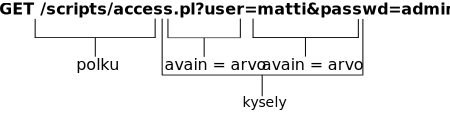
\includegraphics[width=13cm]{pics/logi2.pdf}
\caption{HTTP GET -kyselyn rakenne.}
\label{CLF2}
\end{figure}


\section{Tiedon rakenne}

Web-hotelli, josta data on peräisin, on toteutettu siten, että yksittäiset palvelut on
sijoitettu jokaiselle palvelimelle. Ratkaisun taustalla on
kuormituksen tasaaminen. Erillinen järjestelmä huolehtii siitä, että
Internetistä tulevat kyselyt ohjataan tasaisesti eri
palvelimille. 

Taulukossa \ref{nimet} on esimerkki palveluiden ja
palvelinten nimeämisestä.

% Ei kannata ottaa esimerkkiä tästä taulukosta, tämä on vähän mutkikas.
\begin{table}[h]
\centering
\begin{tabular}{lll}
Palvelin && Palvelu \\
\cline{1-1}\cline{3-3}
dapper && buzz \\
edgy && rex \\
feisty && potato \\
&& hamm \\
\end{tabular}
\caption{Palvelinten ja palveluiden nimeäminen.}
\label{nimet}
\end{table}

Lokitiedostot on sijoitettu hakemistorakenteeseen, jossa juuressa ovat
palvelinten nimien mukaiset hakemistot, joiden sisällä sijaitsevat
lokitiedostot, jotka on nimetään yhdistämällä palvelun nimi
päivämääräleimaan. Tiedostonnimessä käytetty päivämäärän muoto
noudattaa ISO 8601 -standardia~\cite{iso8601}. Tiedostot on pakattu
\texttt{gzip}-pakkausohjelmalla. Taulukossa \ref{tiedostot}
havainnollistetaan tiedostonnimien muodostumista.

\begin{table}[h]
\centering
\begin{tabular}{llll}
Palvelin & Palvelu & Päivämäärä & Tiedostonnimi \\
\hline
edgy & buzz & 14.6.2009 & \texttt{edgy/buzz.http.2009-06-14.gz}\\ 
dapper & potato & 2.7.2009 & \texttt{dapper/potato.http.2009-07-02.gz}\\
feisty & rex & 30.7.2009 & \texttt{feisty/rex.http.2009-07-30.gz}\\
\end{tabular}
\caption{Tiedostojen nimeäminen.}
\label{tiedostot}
\end{table}

Tässä mainittujen palvelinten lisäksi käytössä on ulkoinen
välimuistipalvelu, jonka kautta välitetään harvoin muuttuvia
resursseja, kuten kuvia. Valtaosa dataliikenteestä
välitetään palvelun kautta. Välimuistipalvelu toimii siten, että
mikäli pyydettyä resurssia ei löydy sen omasta muistista, se pyytää
sitä yhdeltä Web-hotellin palvelimista ja välittää vastauksen edelleen
asiakkaalle. Välimuistipalvelun käyttö ei kuitenkaan muilta osin
vaikuta palvelun rakenteeseen. Rakenne käy ilmi kuvasta
\ref{palvelinrakenne}.

\begin{figure}[htp]
\centering
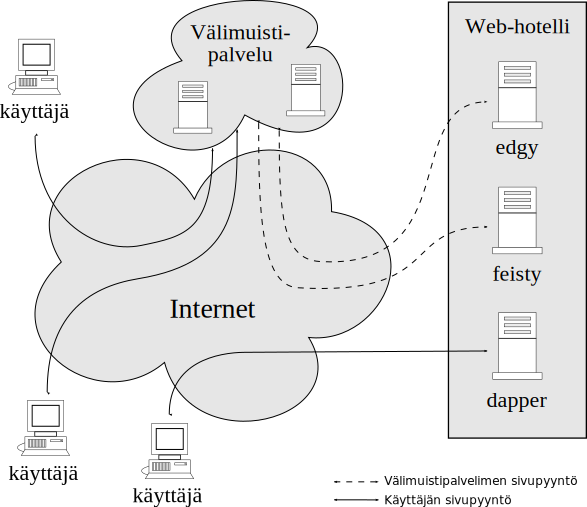
\includegraphics[width=12cm]{pics/palvelinrakenne.pdf}
\caption{Web-palvelun rakenne.}
\label{palvelinrakenne}
\end{figure}

\section{Tavoite}

Tiedon käsittely voidaan jakaa esikäsittelyyn, menetelmään ja
jälkikäsittelyyn. Esikäsittelyn tavoitteena on muuntaa palvelinlokit
muotoon, jota menetelmä pystyy käsittelemään. Menetelmävaiheessa
aineisto ajetaan diffuusiokuvausalgoritmin läpi. Jälkikäsittelyssä
luetaan diffuusiokuvauksen tuottamaa dataa ja selvitetään
mielenkiintoisten havaintojen taustalla olevat HTTP-kyselyt.

\section{Esikäsittely}

Luvussa \ref{sec:lahtokohta} esiteltiin lokitiedostoissa käytetty
\textit{Combined Log Format} -muoto. Tiedosto on tekstimuotoinen,
joten se ei sellaisenaan sovellu analyysivaiheeseen, jossa käsitellään
klustereita. Osa palvelinlokin sisällöstä on myös analyysin kannalta
tarpeetonta ja nämä osat tulee suodattaa pois. Lisäksi yhteen
Web-palveluun liittyvät kyselyt ovat lisäksi jakautuneet useaan eri
tiedostoon eri palvelinten ja vuorokausien mukaisesti.

Esikäsittelijä on toteutettu osana tätä tutkimusta. Esikäsittelijä on
nimeltään \textit{PhasefulSplitter} ja se on toteutettu
Haskell-ohjelmointikielellä~\cite{haskell98}. Haskell tarjoaa
tehokkaat työkalut ohjelmakoodin rinnakkaistamiseen ja datan
sarjallistamiseen. \textit{PhasefulSplitter} on vapaa ohjelma ja sitä saa
levittää edelleen ja muuttaa Free Software Foundationin julkaiseman
GNU General Public Licensen (GPL-lisenssi) version 3~\cite{gplv3} tai (valinnan
mukaan) myöhemmän version ehtojen mukaisesti. Esikäsittelijä on
ladattavissa Internetistä osoitteesta \\
\url{http://iki.fi/zouppen/repo/phasefulsplitter.git}.

Sopivaa yksivaiheista parseria käyttämällä olisi mahdollista käsitellä
lähtödata suoraan analyysissä käytettävään muotoon. Käytännössä
kuitenkin datan esikäsittely kannattaa hoitaa useammassa vaiheessa,
jotta datassa olevat puuttuvat tai poikkeavat arvot voidaan huomioida
ja esikäsittelijää voidaan korjata suorittamatta koko ajoa uudelleen
alusta lähtien. Monivaiheinen esikäsittely helpottaa myös datan
käsittelyä jälkikäteen erilaisin menetelmin. Lisäksi sarjallistetut
tietorakenteet voidaan tarvittaessa anonymisoida, jolloin dataa
voidaan luovuttaa myös ulkopuoliseen käyttöön.

Tiedon käsittelyn helpottamiseksi tässä työssä käytetään esikäsittelyn
välivaiheet ja lopputulokset tallennetaan väliaikaistiedostoihin.
Relaatiotietokantaa ei käytetä, koska tietokantakyselyiden
rinnakkaistaminen osoittautui hyvin vaikeaksi verrattuna suoraan
tiedostoja käsittelevään toteutukseen.

Esikäsittely jakaantuu seuraavaat kolmeen vaiheeseen:

\begin{enumerate}
\item Tiedostolistan muodostaminen ja tiedostojen ryhmittely palveluittain.
\item Tiedostojen sisällön lukeminen ja muuntaminen tietorakenteeksi.
\item Tietorakenteiden jatkokäsittely menetelmälle soveltuvaan muotoon.
\end{enumerate}

\subsection{Tiedostolistan muodostaminen}

Tekstipohjainen tiedostolista luetaan
\textit{PhasefulSplitter}-ohjelman ymmärtämään muotoon, jolloin
tiedostonnimet ryhmitellään palveluiden nimien perusteella. 

Luokittelun yhteydessä palvelinten nimet korvataan numeerisilla
viitteillä. Tätä varten asetetaan tiedestoon \texttt{server.map}
palvelinten nimet ja niitä vastaavat numeeriset viitteet. Viitteitä
voidaan hyödyntää myöhemmin, jos halutaan muuntaa analyysivaiheessa
kiinnostava havainto takaisin Apache-lokin riviksi. Tässä luvun
esimerkissä käytettävän tiedoston sisältö on esitelty listauksessa
\ref{servermap}

\begin{lstlisting}[language=MyHaskell,float=h,caption=Tiedoston server.map sisältö.,label=servermap,aboveskip=1cm]
[
      ("dapper",1)
    , ("edgy",2)
    , ("feisty",3)
]
\end{lstlisting}

Tiedostolista voidaan muodostaa
Linux-järjestelmässä seuraavalla tavalla:

\begin{lstlisting}[language=bashshell]
mkdir lists
find [[polku]] -iname '*.gz' | classifier lists/
\end{lstlisting} 
\label{filelist}

Ajon yhteydessä muodostuu hakemiston \texttt{lists} alle palveluiden
mukaan nimetyt tiedostot. Tiedostomuoto joiden sisällä on palveluun kuuluvat
tiedostonnimet sekä tiedon siitä, minkä palvelimen lokitiedostosta on kyse. Tiedostot ovat tekstimuotoon sarjallistettuja.

\subsection{Muuntaminen tietorakenteeksi}

Toisessa vaiheessa tekstimuotoiset lokitiedostot luetaan ja
käsitellään koneellisesti helpommin analysoitavaan muotoon. Tätä työtä
varten kehitetyssä tiedonkäsittelijässä lokitiedoston rivin eri kentät
palastellaan ja kyselyt sarjallistetaan tiedostoihin. Tietorakenne on
esitelty listauksessa \ref{entry}.

\lstset{language=MyHaskell}

\begin{lstlisting}[float=h,caption=Yhden lokirivin säilövä tietorakenne.,label=entry,aboveskip=1cm]
data Entry = Entry {
      info      :: LineInfo
    , ip        :: ByteString
    , date      :: UTCTime
    , method    :: ByteString
    , url       :: URL
    , protocol  :: ByteString
    , response  :: Integer
    , bytes     :: Integer
    , referer   :: ByteString
    , browser   :: ByteString
} deriving (Show,Eq)
\end{lstlisting}

Koska jatkokäsittely voidaan hoitaa säikeistettynä useammalle
prosessorille tai ytimelle, tässä vaiheessa sovellukselle tulee
ilmoittaa säikeiden määrä. Tiedon perusteella sovellus jakaa yhteen
palveluun liittyvän datan haluttuun määrään erillisiä tiedostoja. Jako
mahdollistaa tehokkaan jälkikäsittelyn, koska tiedostojen sisältöä on
mahdollista käsitellä myöhemmin samanaikaisesti.

Linuxin \texttt{xargs}-komennolla voidaan myös tämän vaihe suorittaa
rinnakkaistettuna, jolloin eri palveluihin kuuluva data voidaan
muuntaa samanaikaisesti. Mikäli eri palveluihin kuuluvien lokien datamäärä
vaihtelee, ei rinnakkaistamisesta kuitenkaan saavuteta täyttä hyötyä.

Alla olevassa esimerkissä esikäsitellään \texttt{lists}-hakemistosta
löytyvät tiedostolistat ja kirjoitetaan ne hakemiston \texttt{data}
alle. Korvaa listauksessa esiintyvä N tietokoneen prosessorien tai
ytimien määrällä. 

\begin{lstlisting}[language=bashshell]
ls lists/*| xargs -n 1 -I{} -P [[N]] apache2data [[N]] {} data/
\end{lstlisting}

Suoritusaika riippuu luonnollisesti koneen suorituskyvystä ja
lokitiedostojen määrästä. Tämän tutkimuksen yhteydessä suoritetussa 24
gigatavun ajossa 2,5 gigahertsin Intel Xeon -prosessorilla varustetussa
tietokoneessa tämän vaiheen suoritus kesti useita
prosessorivuorokausia.

\subsection{Parametrien N-grammianalyysi}

Palvelinlokissa olevista kyselyistä muodostetaan tietorakenne, jossa
yksi osa on kyselyn URL. Tässä vaiheessa tutkitaan URL-osoitetta
tarkemmin. Mikäli URL:n osana on parametreja, muodostetaan jokaisesta
parametrin arvosta 2-grammilistaus. Näin saadut 2-grammikartat
muodostetaan ja lopuksi ne tallennetaan matriisina tekstimuotoon
jatkokäsittelyä varten. Tiedostossa \texttt{ParameterAnalyzer.hs} on
määritelty vakiona, että lasketaan nimenomaisesti 2-grammit. Tätä
vakiota voi kuitenkin tarvittaessa muuttaa.

Ensimmäisessä ajossa selvitetään, mitkä mahdollisista 2-grammeista
ylipäätään esiintyvät aineistossa. Mahdollisia N-grammeja on yhteensä
$2^{8n}$ kappaletta, koska käsiteltävät merkkijonot koostuvat
Word8-tyypeistä (8-bittinen tavu). Säästääkseme muistia
analyysivaiheessa, selvitetään aluksi, millaisia 2-grammeja
aineistossa esiintyy ja jätetään taulukoimatta sellaiset 2-grammit,
jotka eivät esiinny lainkaan.

Jokaiselle resurssille muodostuu oma N-grammilistansa. Datan määrä
luonnollisesti riippuu käytettävästä aineistosta. Käyttämällämme
datalla taulukon kooksi muodostuu muutamia megatavuja (FIXME täsmällisesti).
Lopputulos on kuitenkin vain murto-osa alkuperäisen datamassan
suuruudesta.

N-grammianalyysin ensimmäinen vaihe suoritetaan menemällä halutun
palvelun mukaiseen hakemistoon ja suorittamalla seuraavan komennon:

\begin{lstlisting}[language=bashshell]
parameter_analyzer *.pf.gz +RTS -N
\end{lstlisting} 

Hakemistoon muodostuu ajon seurauksena tiedostot \texttt{ngrams.out}
ja \texttt{grams\_raw.txt}. Näistä ensimmäinen on binaarimuodossa ja
sisältää toisessa vaiheessa tarvittavan datan
binaarimuodossa. Toisessa tiedostossa on tekstimuodossa (Haskellin
show-muodossa) eri resurssien ja 2-grammien
esiintymistiheydet. Tekstimuotoista tiedostoa voidaan käyttää apuna
arvioitaessa, mihin resursseihin ja parametreihin kannattaa kiinnittää
jatkossa huomiota.

Tämän jälkeen voidaan suorittaa n-grammianalyysin toinen vaihe koko
palvelun sisältämälle datalle. Suoritetaan seuraava komento samassa
hakemistossa, missä ensimmäinen vaihekin suoritettiin:

\begin{lstlisting}[language=bashshell]
ghci ParameterToVector.hs
processFile gramFile prefix fromFile
\end{lstlisting} 

Käyttämässämme datassa olevat kyselyiden parametrit sisältävät hyvin
samantyyppisiä arvoja, joten niistä muodostuu kohtuullisen
pieniulotteisia 2-grammitaulukoita. Tässä tutkimuksessa käytetyllä
aineistolla suurin esiintynyt 2-grammien lukumäärä oli
189. Käytännössä havaittiin, että käyttämällämme laitteistolla alle
200 saraketta sisältävän matriisin laskenta oli riittävän
nopeaa. Tämän vuoksi dimensioita ei tarvitse vähentää, joten matriiseihin ei sovelleta
satunnaisprojektiota.


\section{Jatkokäsittely}

Lopuksi eri kenttien  numeeriset arvot Osa arvoista toimii
sellaisenaan klustereina, mutta osa täytyy luokitella.

TODO

Merkkijonoja sisältävät arvot toimivat kukin omana klusterinaan. HTTP
Method -kentässä esiintyvät arvot numeroidaan seuraavasti:

% ["HEAD","GET","POST","PUT","DELETE","TRACE","OPTIONS", "CONNECT","PATCH"]

% ["HTTP/1.0","HTTP/1.1"]

Tässä vaiheessa kuvassa \ref{ngramdata} esiintyvä tietorakenne
muunnetaan matriisimuotoon.

%data ParamInfo = ParamInfo {
%      paramCount :: Integer                    -- ^Frequency of this parameter.
%    , ngramMap   :: M.Map (Ngram Char) Integer -- ^N-grams.
%    } deriving (Show,Read,Eq)

%data ResourceStat = ResourceStat {
%      resourceCount :: Integer                 -- ^Frequency of this resource.
%    , params        :: M.Map String ParamInfo  -- ^Key and its n-gram.
%} deriving (Show,Read,Eq)


TODO

\section{Matlab toteutus}
\label{sec:matlab}

Diffuusikuvausten laskemiseen voidaan käyttää korkeintaan noin 5000 yksittäistä pistettä 2000 pisteen ollessa laskennallisesti vielä tehokasta. Rajoitus johtuu siitä, että
algoritmin aikavaativuus kasvaa eksponentiaalisesti verrattaessa opetusmateriaalin kokoon. 

\section{Pisteen takaisin muuntaminen palvelinlokin riviksi}

LineInfo-tietorakennetta kuljetetaan esikäsittelyvaiheesta
lähtien datan mukana. Tietorakenne tallennetaan matriisin kolmeen
ensimmäiseen sarakkeeseen, eli tekstimuotoisessa esityksessä se
sijaitsee rivin kolmessa ensimmäisessä pilkulla erotetussa kentässä.


kaikki anomaliat kaikissa resursseissa:

%a <- readZipolaFile "/home/joell/zipolalta/service_a_anomalies.csv"
%saveLogLines tiedostolistaus kohde a

%anomaliat resursseittain ryhmiteltynä:

%backtrackCSVnumeric
%tiedostolistaus
%vektorihakemisto
%kohde
%[1,18,337,721,723,882]

TODO

% -*- mode: LaTeX; coding: utf-8; -*-

\chapter{Tiedon analysointi}

\todo{Tämän rakenne on vielä kokonaan miettimättä.}

TODO.

\section{Analysoinnin vaiheet}

Kolmannessa vaiheessa tapahtuu varsinainen analysointi. Käytetty
anomalia-a\-na\-lyy\-si edellyttää, että aineiston muuttujat ovat
luokka-asteikollisia ja tästä johtuen tieto on klusteroitu esikäsittely vaiheessa.

TODO. Tuomon ja Juhon maaginen anomaliamylly tähän.

% -*- mode: LaTeX; coding: utf-8; -*-

\chapter{Yhteenveto}

TODO.


\bibliography{lahteet}{}
%\bibliographystyle{finplain}
\bibliographystyle{ieeetr}

\appendix

%\chapter{Published article}
%
%\includepdf[pages=-]{published_article.pdf}

\end{document}
